\documentclass[10pt,conference]{IEEEtran}

\usepackage{graphicx}
\usepackage{multirow}
\usepackage{ragged2e}
\usepackage{textcomp}
\usepackage{array}
\usepackage{booktabs}
\usepackage{makecell}
\usepackage[table]{xcolor}
\usepackage{color,soul}

\graphicspath{{assets/figures/}}

%\DeclareRobustCommand{\hldel}[1]{{\sethlcolor{red}\hl{#1}}}

\begin{document}

\title{A Comparison of Inertial Data \\ Acquisition Methods for a Position-Independent \\ Soil Types Recognition}

\author{
    \IEEEauthorblockN{
        Florentin Thullier\IEEEauthorrefmark{1},
        Val\`ere Plantevin\IEEEauthorrefmark{1},
        Abdenour Bouzouane\IEEEauthorrefmark{1},
        Sylvain Hall\'e\IEEEauthorrefmark{2} and
        S\'ebastien Gaboury\IEEEauthorrefmark{1}
    }

    \IEEEauthorblockA{
        \IEEEauthorrefmark{1}LIARA Laboratory, Department of Computer Science and Mathematics, \\
        Universit\'e du Qu\'ebec \`a Chicoutimi, Chicoutimi, Qu\'ebec, Canada\\
        $Emails: \left\lbrace florentin.thullier1, valere.plantevin1, abdenour\char`_bouzouane, sebastien\char`_gaboury\right\rbrace@uqac.ca$
    }
    \IEEEauthorblockA{
        \IEEEauthorrefmark{2}LIF Laboratory, Department of Computer Science and Mathematics, \\
        Universit\'e du Qu\'ebec \`a Chicoutimi, Chicoutimi, Qu\'ebec, Canada\\
        $Email: shalle@uqac.ca$
    }}

\maketitle

\begin{abstract}
In a previous work, we presented a method to recognize different soil types based on inertial data generated by a user's gait through a wearable device. Although results we have obtained were encouraging, we judged that this method needed further evaluation. Thus, this paper aims at comparing our previous approach between several acquisition methods. The device was upgraded to a 9-axis IMU and a comparison of this wearable with a mobile phone was also offered. Both the features processing and the classification phases remain unchanged from our previous work to perform a proper comparison. Although this evaluation let us expose a slight improvement in the recognition rate, it allowed us to prove the reliability of our device since the performance obtained with the mobile phone was similar. 

% In a previous work, we presented a method to recognize different soil types based on inertial data generated by a user's gait through a wearable device. Although results we obtained were encouraging, we judged that this method needed further evaluation. Then, this paper aims at comparing our previous approach between several acquisition methods. Firstly, the device was upgraded from a 6 to a 9-axis IMU. These three additional axes let us process the Euler angles to include a comparison between 6, 9 and 12-axis. Moreover, a comparison of such device with a mobile phone was also offered. Both the same set of features, as well as the same two machine learning algorithms (Random Forest and $k$-Nearest Neighbors) were kept from our previous work to perform a proper comparison. The same experiment was reproduced and the results obtained have shown an improved accuracy of 92\% for the 9-axis data records produced with the wearable device. Moreover, the reliability of our device has been proven since the performance with the mobile phone was similar.
\end{abstract}

\begin{IEEEkeywords}
    Soil Types, Recognition, Wearable Object, Mobile Device, IMU, Position-Independent
\end{IEEEkeywords}

\section{Introduction \& Related Work}
\label{sec:introduction}
In the past few years, brand manufacturers have pushed the wearable technology in the forefront of the consumer electronics scene. As a result, in 2014, there was 15\% of mobile devices users employing a wearable device in their daily lives %(\textit{e.g.} smartwatches or fitness band) 
\cite{Nielsen2014}. These devices have, first, brought more sensors than the ones already embedded in current smartphones. Moreover, the increasing use of the Bluetooth Low Energy (BLE) technology \cite{Taplett} allowed a more efficient communication with mobile devices as regards energy consumption. In that sense, wearable devices become widely adopted in order to track activities since they present a convenient and portable way to record physiological data produced by their users. Hence, a considerable amount of data is collected each day and several statistical analyses are offered for monitoring carriers' daily activities \cite{Patel2015}. Besides, according to recent advancements in machine learning, it is possible to say that existing activity tracking applications may be enhanced to become more ubiquitous. % (applications that aim to make devices more mobile and smart).

The idea of recognizing soil-type, also known as terrain classification, through data produced by an accelerometer, firstly comes from the mobile robotics area. First of all, Vail and Veloso \cite{Vail2004} experimented a surface detector using inertial data generated by a four-legged robot. Authors opted for a C4.5 decision tree, and they obtained an overall accuracy of 84.9\% over a 10-fold cross-validation method.

% The idea of recognizing soil-type, also known as terrain classification, through data produced by an accelerometer, firstly comes from the mobile robotics area. First of all, Vail and Veloso \cite{Vail2004} experimented a surface detector using inertial data generated by a four-legged robot. Authors opted for a C4.5 decision tree since it is fast enough and simple to represent. In order to quantify the accuracy of their learning model, they used a 10-fold cross-validation method which gives us an overall accuracy of 84.9\% (cement: 91\%; carpet: 81.2\%; field: 81.2\%).

Additionally, Bibuli \textit{et al.} \cite{Bibuli2007} suggested a terrain classification method for a four-wheels mobile robot equipped with several sensors, including inertial ones. Their artificial neural network trained with Discrete Fourier Transform components achieved at best an overall recognition rate of 82.7\% for the x-axis of the gyroscope.

% Additionally, Bibuli \textit{et al.} \cite{Bibuli2007} suggested a terrain classification method for a four-wheels mobile robot equipped with several sensors, including inertial ones. The terrain classification was performed by providing frequency components of the signal, obtained through the Discrete Fourier Transform (DFT), as inputs of an artificial neural network (ANN). Moreover, since they trained one ANN by distinct axis, most valuable results were obtained with the training of the x-axis of the gyroscope, being respectively, 90\%, 71.2\%, 70\%, 98.8\% and 83.5\% for the gravel, grass, sand, pavement and dirt terrains.

In the same way, Weiss \textit{et al.} \cite{Weiss2007} proposed a comparison of terrain recognition for a four-wheeled robot between the Support Vector Machine (SVM) and several other classification techniques. Input data for the SVM algorithm were either a log-scaled Power Spectral Density, or a 128-point Fast Fourier Transform (FFT) features vector. Authors performed the experiment over different velocities of the robot (\textit{i.e.} 0.2, 0.4 and 0.6 m/s) and they obtained most accurate results with SVM rather than other algorithms, such as Probabilistic Neural Network, $k$-Nearest Neighbors ($k$-NN), Na\"ive Bayes and C4.5.

Conversely, Kert\'esz \cite{Kertesz2016} recently introduced a rigidity-based surface recognition for a four-legged robot using features extracted through the FFT, then, classified with the Random Forest (RF) algorithm. Through a 10-folds cross validation method authors have obtained an accuracy of 96.2\%.
% The model was evaluated thanks to the 10-folds cross validation method. The author found that the Random Forest outperformed every other algorithms it was compared to, as he obtained an accuracy of 96.2\%.

Although such a related literature was relevant in understanding how to answer hypotheses we formulated, all of these methods are not suitable for soil-types-recognition in a human-walking context. However, such an idea may also be employed with human beings since several use cases of terrain classification in this context are noticeable to us. For example, we can mention the annotation of every subset of a full GPS trace with a given type of soil for hikers. Another example is related to health since such a recognition may be employed for fall prevention since it is known that it exists more risks when people are walking on certain types of soil. Based in such a postulate, a recent study suggested by Otis \textit{et al.} \cite{Otis2016} introduced a terrain discrimination analysis to reduce the risk of falling through a three-axis accelerometer embedded in a shoe. A clustering algorithm was employed in order to segment FFT-based discriminating features. This work claims a misidentification rate between 1\% and 5\% in a laboratory setup, while it rose up to 20\% in real conditions.

% \hl{Finally, in our previous work {\cite{Thullier2017b}} we introduced a novel method for recognizing soil types based on inertial data produced by users' gait. To achieve this we designed a new wearable device based on the \textit{Arduino 101} board that embed a 6-axis IMU. Several well-known features from both time and frequency domains were computed over each signal to produce discriminating characteristics, then, classified with both the $k$-Nearest Neighbors and the Random Forest algorithms. The model was evaluated thanks to the 10-folds cross validation method and the most valuable results have shown a 87\% accuracy with 9 participants involved. Moreover, this work has proved that the results were not affected regardless of where the device is positioned. However since only data produced by a 6-axis IMU were considered, the results obtained needed to be compared with other acquisition methods to better determine whether the performance of the recognition will increase, or reduce when using more axis.}

% To this end, this work first aims at comparing these results with another sensor capable of providing the measurement of the magnetism. Then, the last objective of this work is to ensure the reliability of the wearable device by comparison with the use of a mobile phone also capable to provide data generated by a 9-axis inertial sensor.

The rest of the paper is structured as follows: section 2 details the suggested method for soil type recognition. Next, section 3 describes experiments we conducted. Section 4 and Section 5 expose and discuss results we obtained. Finally, section 6 draws a conclusion and provides future works.

% The rest of the paper is structured as follows: section 2 details the suggested method for soil type recognition based on inertial data. Next, section 3 describes experiments we conducted in order to compare the different data acquisition methods. Section 4 and Section 5 exposes and discusses results we obtained. Finally, section 6 draws a conclusion and section 7 provides future works.

\section{Proposed Solution}
% This section describes in detail the solution we suggest to perform an empiric comparison of our previous work {\cite{Thullier2017b}} with an upgraded version of the wearable device and the involvement of a mobile phone. % The first two subsections explain both the improved version of the wearable device, and the mobile phone hardware and software configurations. Then, we recall which discriminating features that are computed over raw data, as well as the classification algorithms we kept from our previous work to achieve the recognition of different soil types.

\subsection{Wearable Device}
In order to test our approach and record several datasets, we have conserved the design of the wearable device introduced in \cite{Thullier2017b}. It is based on the % latest \textit{Intel Curie} board from \textit{Arduino}, 
the \textit{Arduino 101} board, with a dedicated proto-shield providing a SD card slot, on which a new 9-axis IMU (\textit{LSM9DS1}) has been installed. % , as shown in Figure \ref{fig:device}.
Our decision in conserving this design was motivated, at first, by the capability of the \textit{Arduino} board to communicate through BLE since it is embedded in many smartphones {\cite{Taplett}} and it offers a very low power consumption {\cite{Gomez2012}}. Secondly, this board offers a large amount of I/O that allows interfacing other hardware. %, for example, either an SD card for large storage or a \textit{LSM9DS1} 9-axis IMU. 
Our custom firmware embedded on the device remains unchanged except that a computation process of the Euler angles was included in the \textit{dataset formatting module}. The inertial data were further obtained at a stable frequency of 60 Hz.

% \begin{figure}[!ht]
%   \centering
%   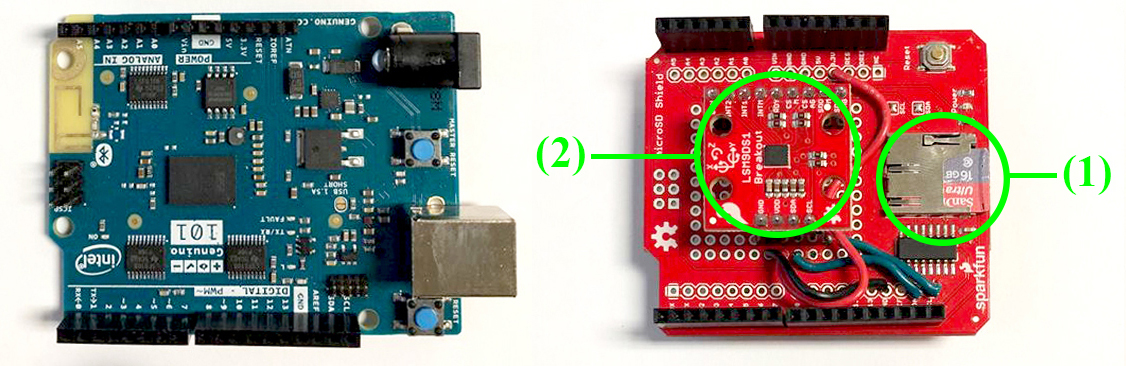
\includegraphics[width=2.4in]{device.jpg}
%   \caption{\textit{Arduino 101} board and the dedicated proto shield with SD card slot (1), as well as the \textit{LSM9DS1} 9-axis IMU (2).}
%   \label{fig:device}
% \end{figure}

%Our decision in conserving this design was motivated by the same reasons as the the previous ones. Fristly, for the capability of the \textit{Arduino} board to communicate through Bluetooth Low Energy (BLE), a wireless technology embedded in many smartphones {\cite{Taplett}}, which offers a very low power consumption {\cite{Gomez2012}}. Secondly for the amount of Inputs/Outputs (I/O) offered by the board that allow interfacing other hardware, for example, either an SD card for large storage or a \textit{LSM9DS1} 9-axis IMU. In that sense, the firmware {\cite{Plantevin2016}} that was embedded on the device in the first place remains unchanged for this work and let us obtain values from the \textit{LSM9DS1} IMU at a stable frequency of 60 Hz.

%Its graphical representation is recalled in Figure \ref{fig:hardware}. The first main component is the command module that is in charge of all the communications between a mobile device and the hardware through the BLE radio module. The second main component is the IMU  recorder. Its goal is to store in a buffer, values coming from the \textit{LSM9DS1} IMU over an I\textsuperscript{2}C bus, at a stable frequency of 60 Hz. It differ from the previous device where the 6-axis IMU embedded in the \textit{Arduino 101} board was communicating over an SPI bus. Finally, the buffer sends all its values, on which Euler angles are processed, in the dataset formatting module at every second. This component takes all the configuration parameters from the command module and creates formatted strings that are written on the memory card. 

% \begin{figure}[!ht]
%   \centering
%   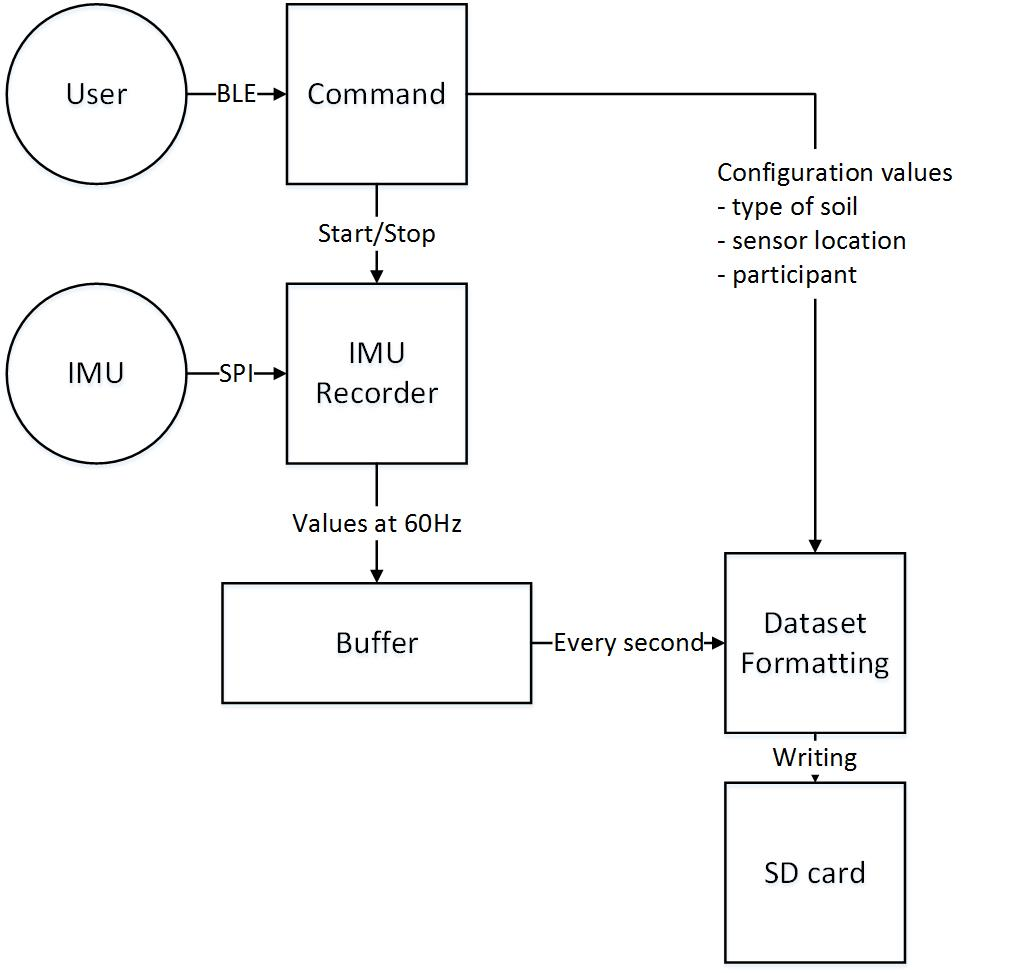
\includegraphics[width=2.8in]{software.jpg}
%   \caption{Graphical representation of the firmware implementation embedded in the wearable device.}
%   \label{fig:hardware}
% \end{figure}

\subsection{Mobile Device}
To compare our wearable device with a mobile phone, a dedicated application was developed to record the values of the embedded 9-axis IMU. Such a record was achieved on a \textit{Huawei Nexus 6P} running \textit{Android} 8.0 and a stable frequency of 60 Hz was also set for this setup. As for our wearable device, the three Euler angles were calculated and finally, all data were stored in the flash memory of the phone.

% To compare the acquisition of inertial data generated by our wearable device with inertial data that came from a mobile phone, an Android application was specially developed. This application was in charge of recording all the values produced by the 9-axis IMU embedded in the phone (\textit{i.e.} \textit{Huawei Nexus 6P} running the 8.0 version of \textit{Android}) at the same stable frequency as the one offered by our wearable device (\textit{i.e.} 60 Hz). For each data coming from the IMU, the three Euler angles are calculated and this set of twelve values is temporarily stored in a buffer. Its content is finally formatted with configuration values and written on the flash memory of the mobile phone at every second, in the same format as for the wearable device.

\subsection{Features Extraction}
The features' extraction process suggests conserving the same set of either time and frequency domain features from our previous work {\cite{Thullier2017b}} that are all computed from a fixed non-overlapping time window over each raw signal. The conversion from the time domain to the frequency one was achieved through the FFT algorithm.

% Following the recording phase, a features extraction process must be done before achieving any classification. We conserved the same features, either from the time or the frequency domain, as in our previous work {\cite{Thullier2017b}}. They are all computed from a fixed non-overlapping time window over each raw signal and the conversion from the time domain to the frequency one was achieved through the FFT algorithm.

% Following the recording phase, where raw data produced by the IMU were collected, a features extraction process must be achieved before classify them with machine learning algorithms. In that sense, we concerve the same set as in our previous work \cite{Thullier2017b} that were selected according to the related litterature \cite{Bussmann2001, Bayat2014, Cleland2013, Kwapisz2011, Yang2008, Ravi2005, Shoaib2013, Gao2014}. These features from either the time or the frequency domain. They are all computed from a fixed non-overlapping time window over each raw signal and the conversion from the time domain to the frequency one was achieved through the Fast Fourier Transform (FFT) algorithm. As examples, the whole set of such features includes the processing of the $skewness$ (\ref{eq:skewness}), the $kutosis$ (\ref{eq:kurtosis}) and the Energy (\ref{eq:energy}).   

%On the first hand, the time-related ones are composed of 11 statistical computations. The first operation is a simple unweighted mean on each axis for each sensor (\textit{i.e.} gyroscope and accelerometer). Then, the average of these values for each specific sensor is processed. In the exact same way, we apply few more statistical calculations: the standard deviation, the \textit{skewness}, the \textit{kurtosis}, the \textit{Zero-crossing rate} and finally, the correlation between all possible axis combinations. Formulas of the $skewness$ and the $kutosis$ measures, when applied to the $W$ axis are respectively reminded in (\ref{eq:skewness}) and (\ref{eq:kurtosis}). In both cases, $N$ represents the number of elements in the vector, $w_i$ is the $i^{th}$ element in it, $\bar{W}$ is the mean of the vector and $\sigma_w$ refers to its standard deviation. Finally, we calculate the correlation between each axis combination from the same sensor as recalled by (\ref{eq:correlation}).

% \begin{equation}
%     \label{eq:skewness}
%     skw(W) = \frac{N}{(N-1)(N-2)}\cdot\left(\sum_{i=1}^{N}{\frac{(w_i-\bar{W})^3}{\sigma_w^3}}\right)
% \end{equation}

% \begin{equation}
%     \label{eq:kurtosis}
%     \resizebox{.9\columnwidth}{!}
%     {
%         $kurtosis(W) = \frac{N(N+1)}{(N-1)(N-2)(N-3)}\cdot\left(\sum_{i=1}^{N}{\frac{(w_i-\bar{W})^4}{\sigma_w^4}-\frac{3(N-1)^2}{(N-2)(N-3)}}\right)$
%     }
% \end{equation}

% \noindent where $W$ is a given axis, $N$ represents the number of elements in the vector, $w_i$ is the $i^{th}$ element in it, $\bar{W}$ is the mean of the vector and $\sigma_w$ refers to its standard deviation.

% \begin{equation}
%     \label{eq:correlation}
%     \rho(U,V) = \frac{cov(U,V)}{\sigma_u\cdot\sigma_v}
% \end{equation}

%On the second hand, several attributes required to be v. In order to achieve such a conversion, the Fast Fourier Transform (FFT) algorithm has been used. These three features are the DC component, the Entropy of each axis frequency representation and finally, the Energy that is defined in (\ref{eq:energy}), where $W$ represents a vector of complex numbers, $N$ refers to its size and $w_i$ is the $i^{th}$ element in it.

% \begin{equation}
%     \label{eq:energy}
%     Energy(W) = \frac{1}{N}\cdot\left(\sum_{i=1}^{N}|w_i|\right)
% \end{equation}

% \noindent where $W$ represents a vector of complex numbers, $N$ refers to its size and $w_i$ is the $i^{th}$ element in it.

\subsection{Classification}
% The last task that must be achieved by our system is a classification process. 
According to the literature in the field of activity recognition, as well as terrain classification in robotics, it is known that several of such algorithms achieve excellent results in classifying data from inertial sensors. This research retains the direct comparison between the RF and the $k$-NN algorithms. This choice was previously made, first because they belong to two distinct families of classifiers\textemdash respectively, the meta-classifiers and the lazy learning ones. Moreover, as non-parametric methods, these algorithms remain simple, flexible, powerful and efficient \cite{Russell2010}. Indeed, their satisfying classification performance is, most of the time, reported in the literature \cite{Kertesz2016, Vail2004}.

% Once discriminating features extracted from raw inertial data are computed, the following task that must be achieved by our system is a classification process. According to the literature in the field of activity recognition, as well as terrain classification in robotics, it is known that several of such algorithms achieve excellent results in classifying data from inertial sensors. As examples, we can mention: Decision Trees (DT), $k$-Nearest Neighbors ($k$-NN), Support Vector Machines (SVM), Artificial Neural Networks (ANN), and Na\"ive Bayes \cite{Tuncel2009, Kertesz2016, Weiss2007, Kim2010, Vail2004, Hoffmann2014, Bibuli2007}. 

% In that sense, this research retain the direct comparison between the Random Forest and the $k$-Nearest Neighbors algorithms. This choice was previously made, first because they belong to two distinct families of classifiers\textemdash respectively, the meta-classifiers and the lazy learning ones. Moreover, as non-parametric methods (methods that do not make strong assumptions about the form of the mapping function), these algorithms remains simple, flexible, powerful and efficient \cite{Russell2010}. Indeed, their satisfying classification performance is, most of the time, reported in the literature \cite{Kertesz2016, Vail2004}.

% \subsubsection{Random Forest}
% According to Breiman \cite{Breiman2001}, a Random Forest (RF) is a combination of tree predictors, where each tree depends on the values of a random vector, sampled independently and with the same distribution for all trees in the forest. The final decision is made by a majority vote between each outcome of each single tree that forms the forest. Figure \ref{fig:rf} exposes a simple example of a Random Forest classification using three trees. Such a classification algorithm implies several initial parameters. The three most important ones which are necessary to define are first, the number of trees in the forest ($B$), second, the number of features to consider when looking for the best split ($F$) and the function used to measure the quality of such a split ($C$). According to the literature, Breiman \cite{Breiman2001} suggests using $F=log_2(m) + 1$ where $m$ refers to the number of attributes present in the dataset. However, it is also possible to find other recommendations such as $F=\frac{1}{2}\sqrt{m}$ or $F=\sqrt{m}$. As regards the quality of the split, the two primary function often employed are first, the calculation of the Gini index and second, the evaluation of the information gain that are respectively expressed by (\ref{eq:gini}) and (\ref{eq:gain}):

% \begin{equation}
%     \label{eq:gini}
%     Gini(T) = {1-\sum_{i=1}^{n}(p_i)}^2
% \end{equation}

% \begin{equation}
%     \label{eq:gain}
%     E(T) = \sum_{i=1}^{n}-(p_i log_2 p_i)
% \end{equation}

% \noindent where $T$ are input data containing instances of $n$ classes and $p_i$ is the relative frequency of class $i \in n$ in $T$. However, this criterion depends essentially of the type of trees that are used in the construction of the forest (\textit{i.e.} ID3, C4.5, CART, \textit{etc.}).

% \begin{figure}[!ht]
%     \centering
%     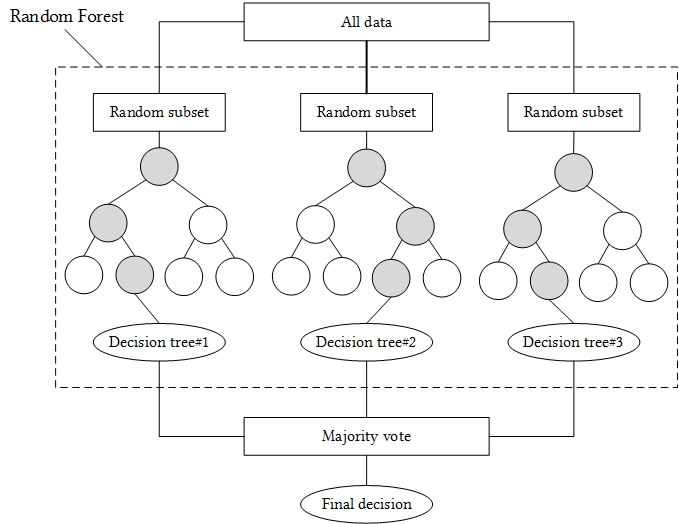
\includegraphics[width=2.8in]{rf.jpg}
%     \caption{A simple example of a Random Forest classification using $B = 3$ trees.}
%     \label{fig:rf}
% \end{figure}

% \subsubsection{$k$-Nearest Neighbors}
% Firstly, this algorithm is a non parametric classification algorithm. In other words, it does not make any assumption on the underlying data distribution. Moreover, it is a lazy algorithm which means that there is no training phase, or it is very minimal. Although $k$-NN is a very fast algorithm, the final classification decision is made based on the entire training dataset that necessarily involve to have some storage space. Indeed, it assumes that the data are in a feature space since they may be scalars or multidimensional vectors. The $k$ closest vectors are extracted by using a distance measure and classes of new unknown data are defined through a majority vote between the label of each class of these $k$ neighbors. Figure \ref{fig:knn} shows a simple example of such a classification when $k=3$ nearest neighbors.

% \begin{figure}[!ht]
%   \centering
%   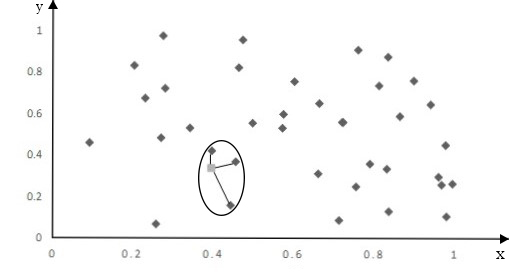
\includegraphics[width=2.8in]{knn.jpg}
%   \caption{A simple example of a 3-Nearest Neighbors classification.}
%   \label{fig:knn}
% \end{figure}

% Once the parameter $k$ is set, it is also important to select the proper distance measure to use for obtaining the $k$ closest vectors. Here, we describe two well-known distance measures: the Euclidean (\ref{eq:d_eucl}) and the Manhattan (\ref{eq:d_manh}) ones. 

% \begin{equation}
% 	\label{eq:d_eucl}
% 	D_{Euclidean} = \sqrt{\sum_{i=1}^{n}(u_i-v_i)^2}
% \end{equation}

% \begin{equation}
% 	\label{eq:d_manh}
% 	D_{Manhattan} = \sum_{i=1}^{n}\left|u_i-v_i\right|
% \end{equation}

\section{Experiments}
% Experiments we have conducted involved, several participants that are described in the first point of this section. Moreover, both the requirements of the experiment and the procedure of the data collection are described in the two following subsections. 

\subsection{Participants}
Since our previous work, only six over the nine recruited participants were available. They were all the same university students, being all males from 23 to 30 years old. Their weights were placed between 65 kg and 110 kg (median: 85 kg), and their heights were between 172 cm and 192 cm (median: 181 cm) respectively. Moreover, we counted up 5 right-handed persons and 1 left-hander. All of them were healthy people without any motor function issues.

\subsection{Requirements}
In order to preserve the consistency of the experiment previously proposed, the 215 cm long and 90 cm wide box was reused at it was (filled with either gravel or sand). Nevertheless, because of the time of the year, the data collection was impossible to reproduce on the snow.

%On the first hand, since our University is located in a region with hard weather conditions, most of the different soil types are recovered either, or both, of ice or snow. To cope with such an issue, we have built a box which was filled with few of the most common soil types that is possible to find outside (\textit{i.e.} gravel and sand). The box was 215 cm long and 90 cm wide as shown on Figure \ref{fig:box}. This requirement was kept from our previous research to preserve the consistency of the experiment. However, because of the time of the year, the data collection was impossible to reproduce on the snow.

% \begin{figure}[!ht]
%   \centering
%   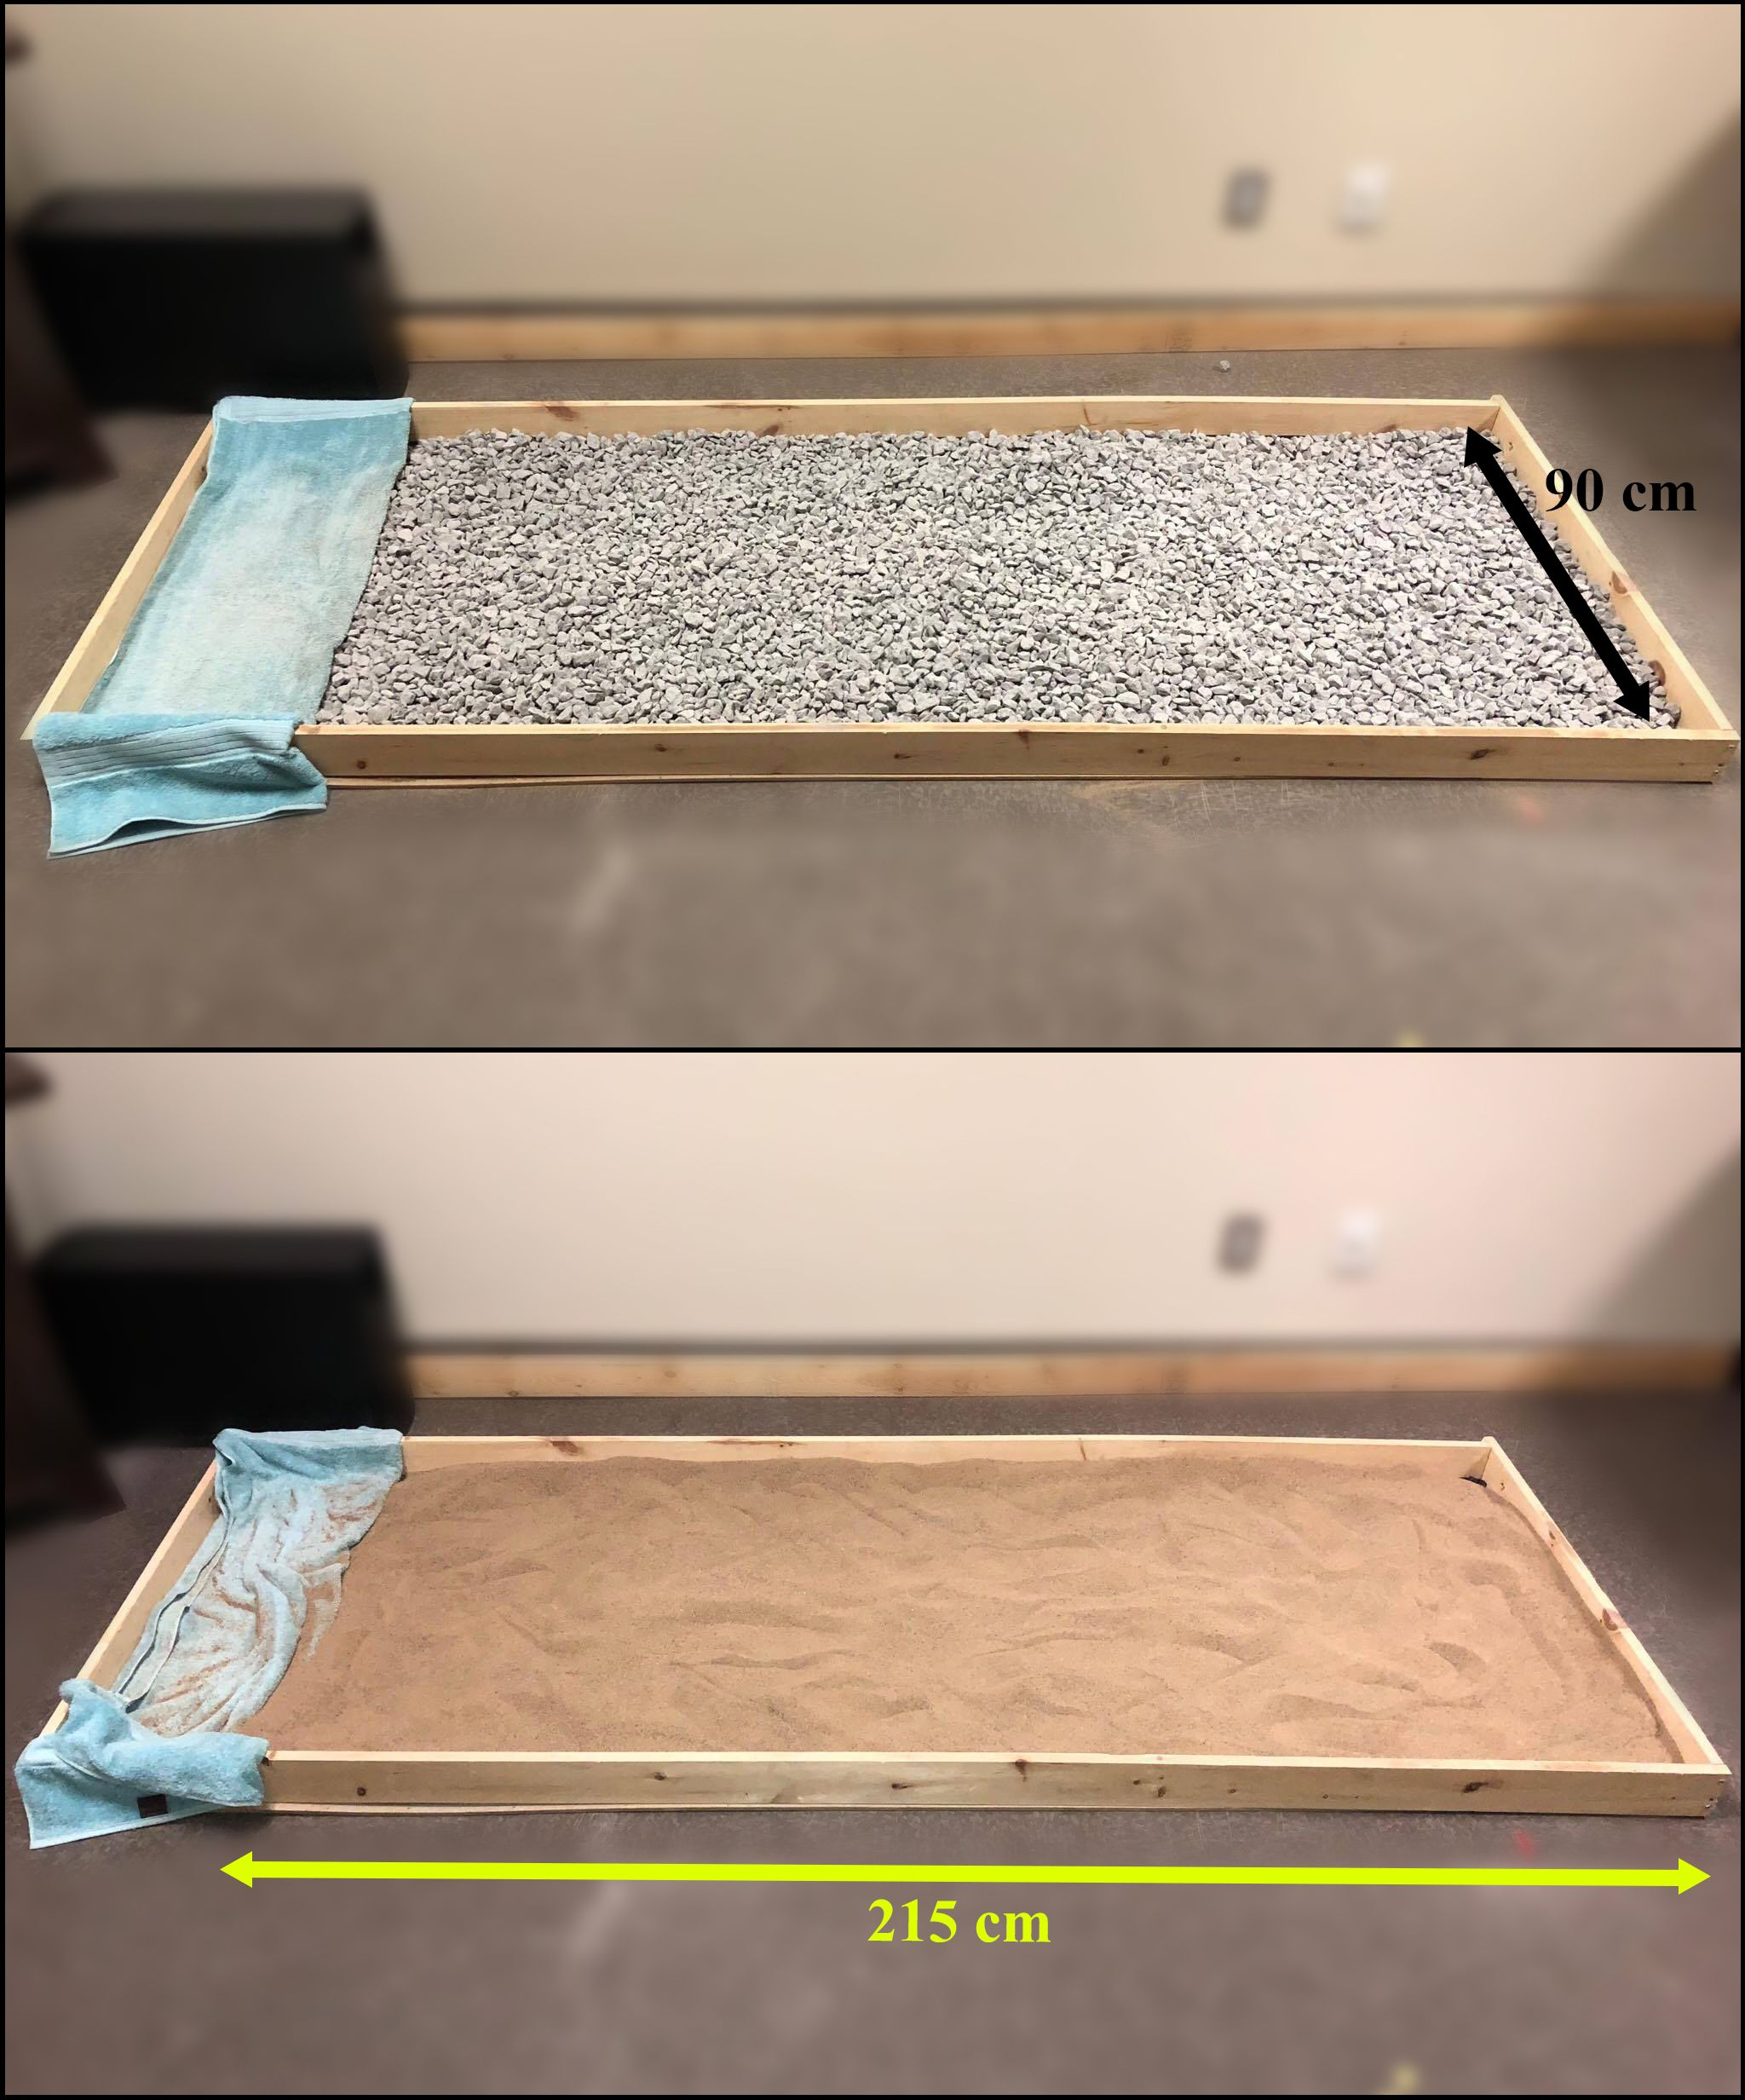
\includegraphics[width=2.2in]{box.jpg}
%   \caption{The box used for our experiments filled first with gravel and then with sand.}
%   \label{fig:box}
% \end{figure}

% On the second hand, we needed to tell both the wearable device and the mobile device when to start and stop, and how to annotate correctly each record. To this end, we concerved the \textit{Android} application we developed to pilot our wearable device suggested in our previous research {\cite{Thullier2017b}}. The same phone (\textit{LG Nexus 5} with the 6.0.1 version of \textit{Android}) was used to run this application. Hence, the mobility allowed by the smartphone instead of a traditional desktop computer application was preserved.

% Since the wearable device provide a Bluetooth Low Energy (BLE) connectivity, the first task to perform with the application is to scan all the devices available in this area and to pair with ours through the application. %, as exposed in the first screen of the Figure \ref{fig:android_app}. 
% Then, the second screen shows the interface that allowed us to annotate each record with the following information: the soil type on which the user is about to walk, the position of the wearable device (within: \textit{backpack}, \textit{left} and \textit{right hand bag}, and \textit{left} and \textit{right pocket}), as well as the identification of the current participant (where each one was anonymized by a capital letter).

The management of the recording was synchronized to start and stop the data collection for the two devices at the same time. Moreover, the annotation of all the records was done similarly to our previous work through the same \textit{Android} application {\cite{Thullier2017b}}, where each participant was anonymized by the same capital letter for every of their records.

% \begin{figure}[!ht]
%   \centering
%   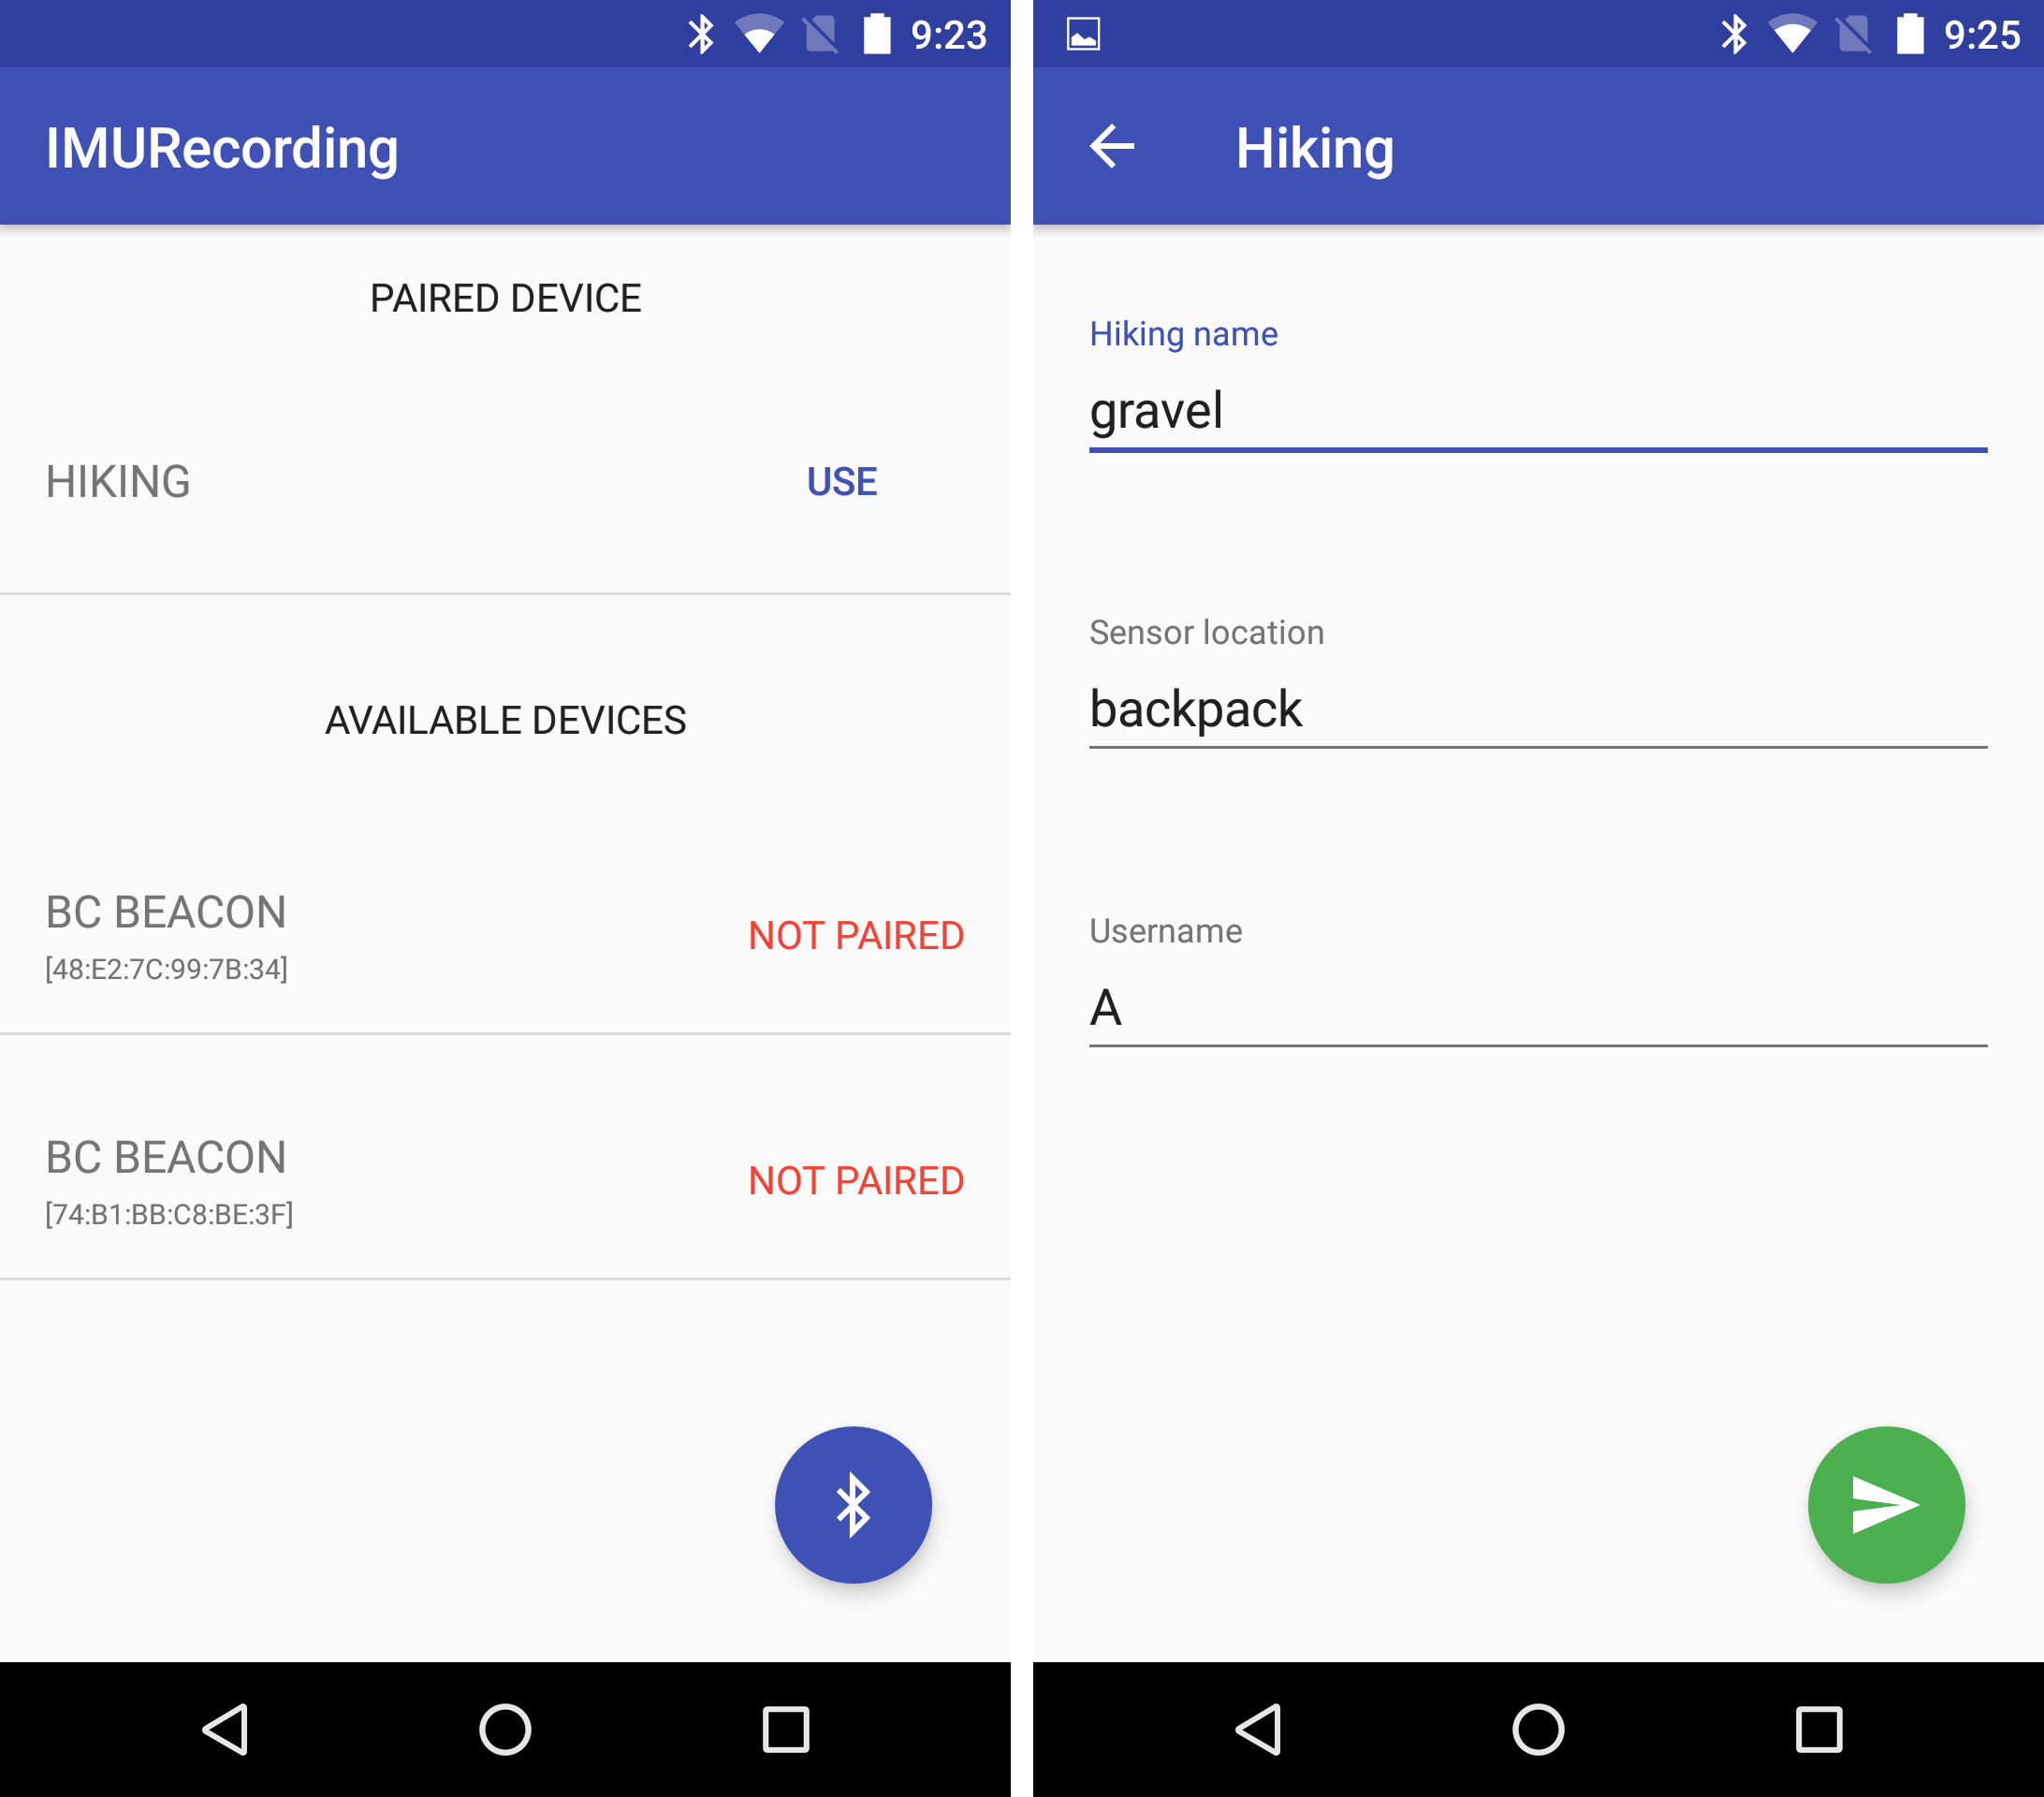
\includegraphics[width=2.5in]{android_app.jpg}
%   \caption{Screens of the Android application which was used to pair with the device and pilot the annotation of the inertial data records.}
%   \label{fig:android_app}
% \end{figure}

\subsection{Procedure}
To perform the data collection, we attempted to get as close as possible to real use case situations. In that sense, we judge that the three most natural places where a user may wear the device are: a hand-bag, a backpack and inside the pockets of a jacket. Both the hand-bag and the backpack were ballasted with an extra weight (1 kg and 3 kg respectively) as they could be in real use case scenarios. 
% However, since we wanted to determine the impact of the location of both devices accurately, participants were asked to wear both devices at the same time on the right and the left shoulder for the hand-bag. Such a bag was ballasted with an extra weight of 1 kg. In the same way, participants were requested, to wear both devices inside the right and the left pockets of the jacket. 
Moreover, since we wanted to reduce variable noise that may occur due to arm balancing, a special attention was placed on preserving the jacket closed during each walk.


%, as shown in Figure \ref{fig:positions_hand_bags}. 

% \begin{figure}[!ht]
%   \centering
%   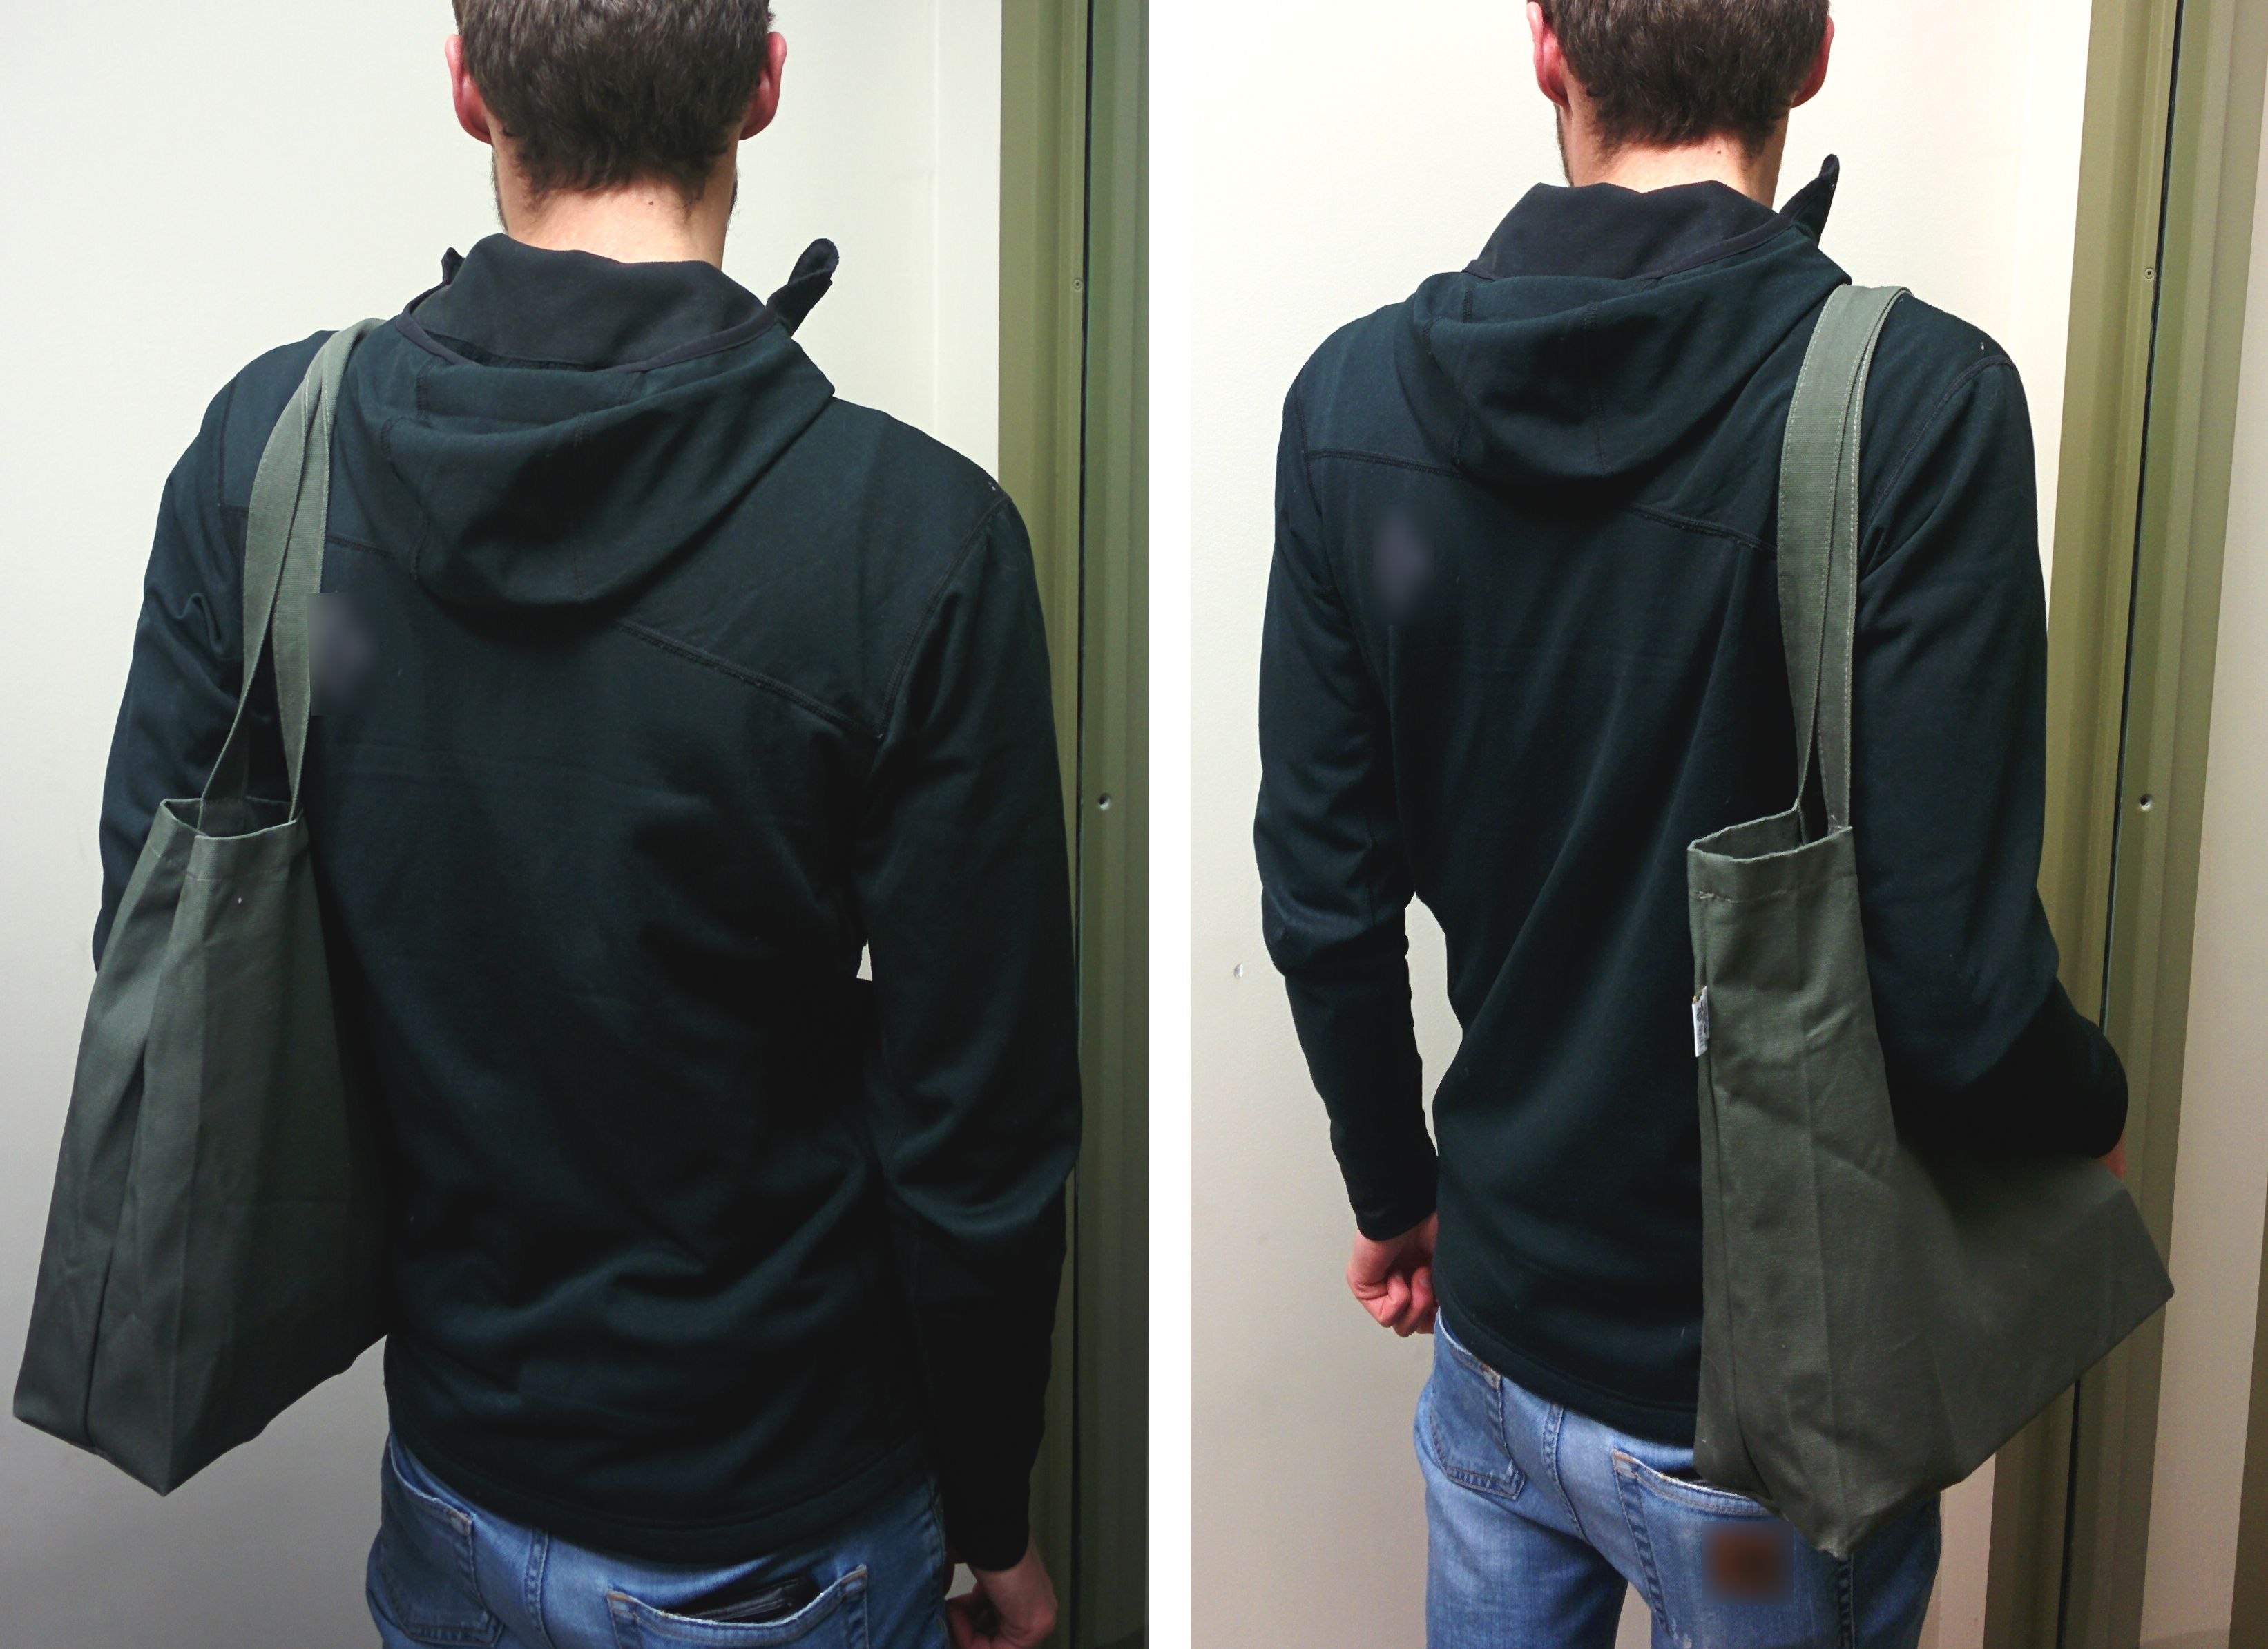
\includegraphics[width=2.8in]{positions_hand_bags.jpg}
%   \caption{Position of the wearable device inside the hand bag being both on the left and the right shoulder.}
%   \label{fig:positions_hand_bags}
% \end{figure}

%Moreover, 
% Such a bag was ballasted with an extra weight of 1 kg. In the same way, participants were requested, to wear both devices inside the right and the left pockets of the jacket. %, as illustrated in the left of Figure \ref{fig:positions}
% Since we wanted to reduce variable noise that may occur due to arm balancing, a special attention was placed on preserving the jacket closed during each walk.

%, where v. We have formulated such a requirement in order to reduce variable noise that may have been created on inertial data because of the proper arm balancing of each participant. Finally, the last position we have experienced here concerns the positioning inside a standard 20 L hiking backpack which weighed approximately 3 kg.
% , where a special attention was placed on preserving the jacket closed during each walk. We have formulated such a requirement in order to reduce variable noise that may have been created on inertial data because of the proper arm balancing of each participant. Finally, the last position we have experienced here concerns the positioning inside a standard 20 L hiking backpack which weighed approximately 3 kg. % The wearable device was placed inside the largest pocket in the same direction for each participant, while the mobile device was placed in the front zipper of the bag also in the same direction for each walker. % as demonstrated in the right of the Figure \ref{fig:positions}.

% \begin{figure}[!ht]
%   \centering
%   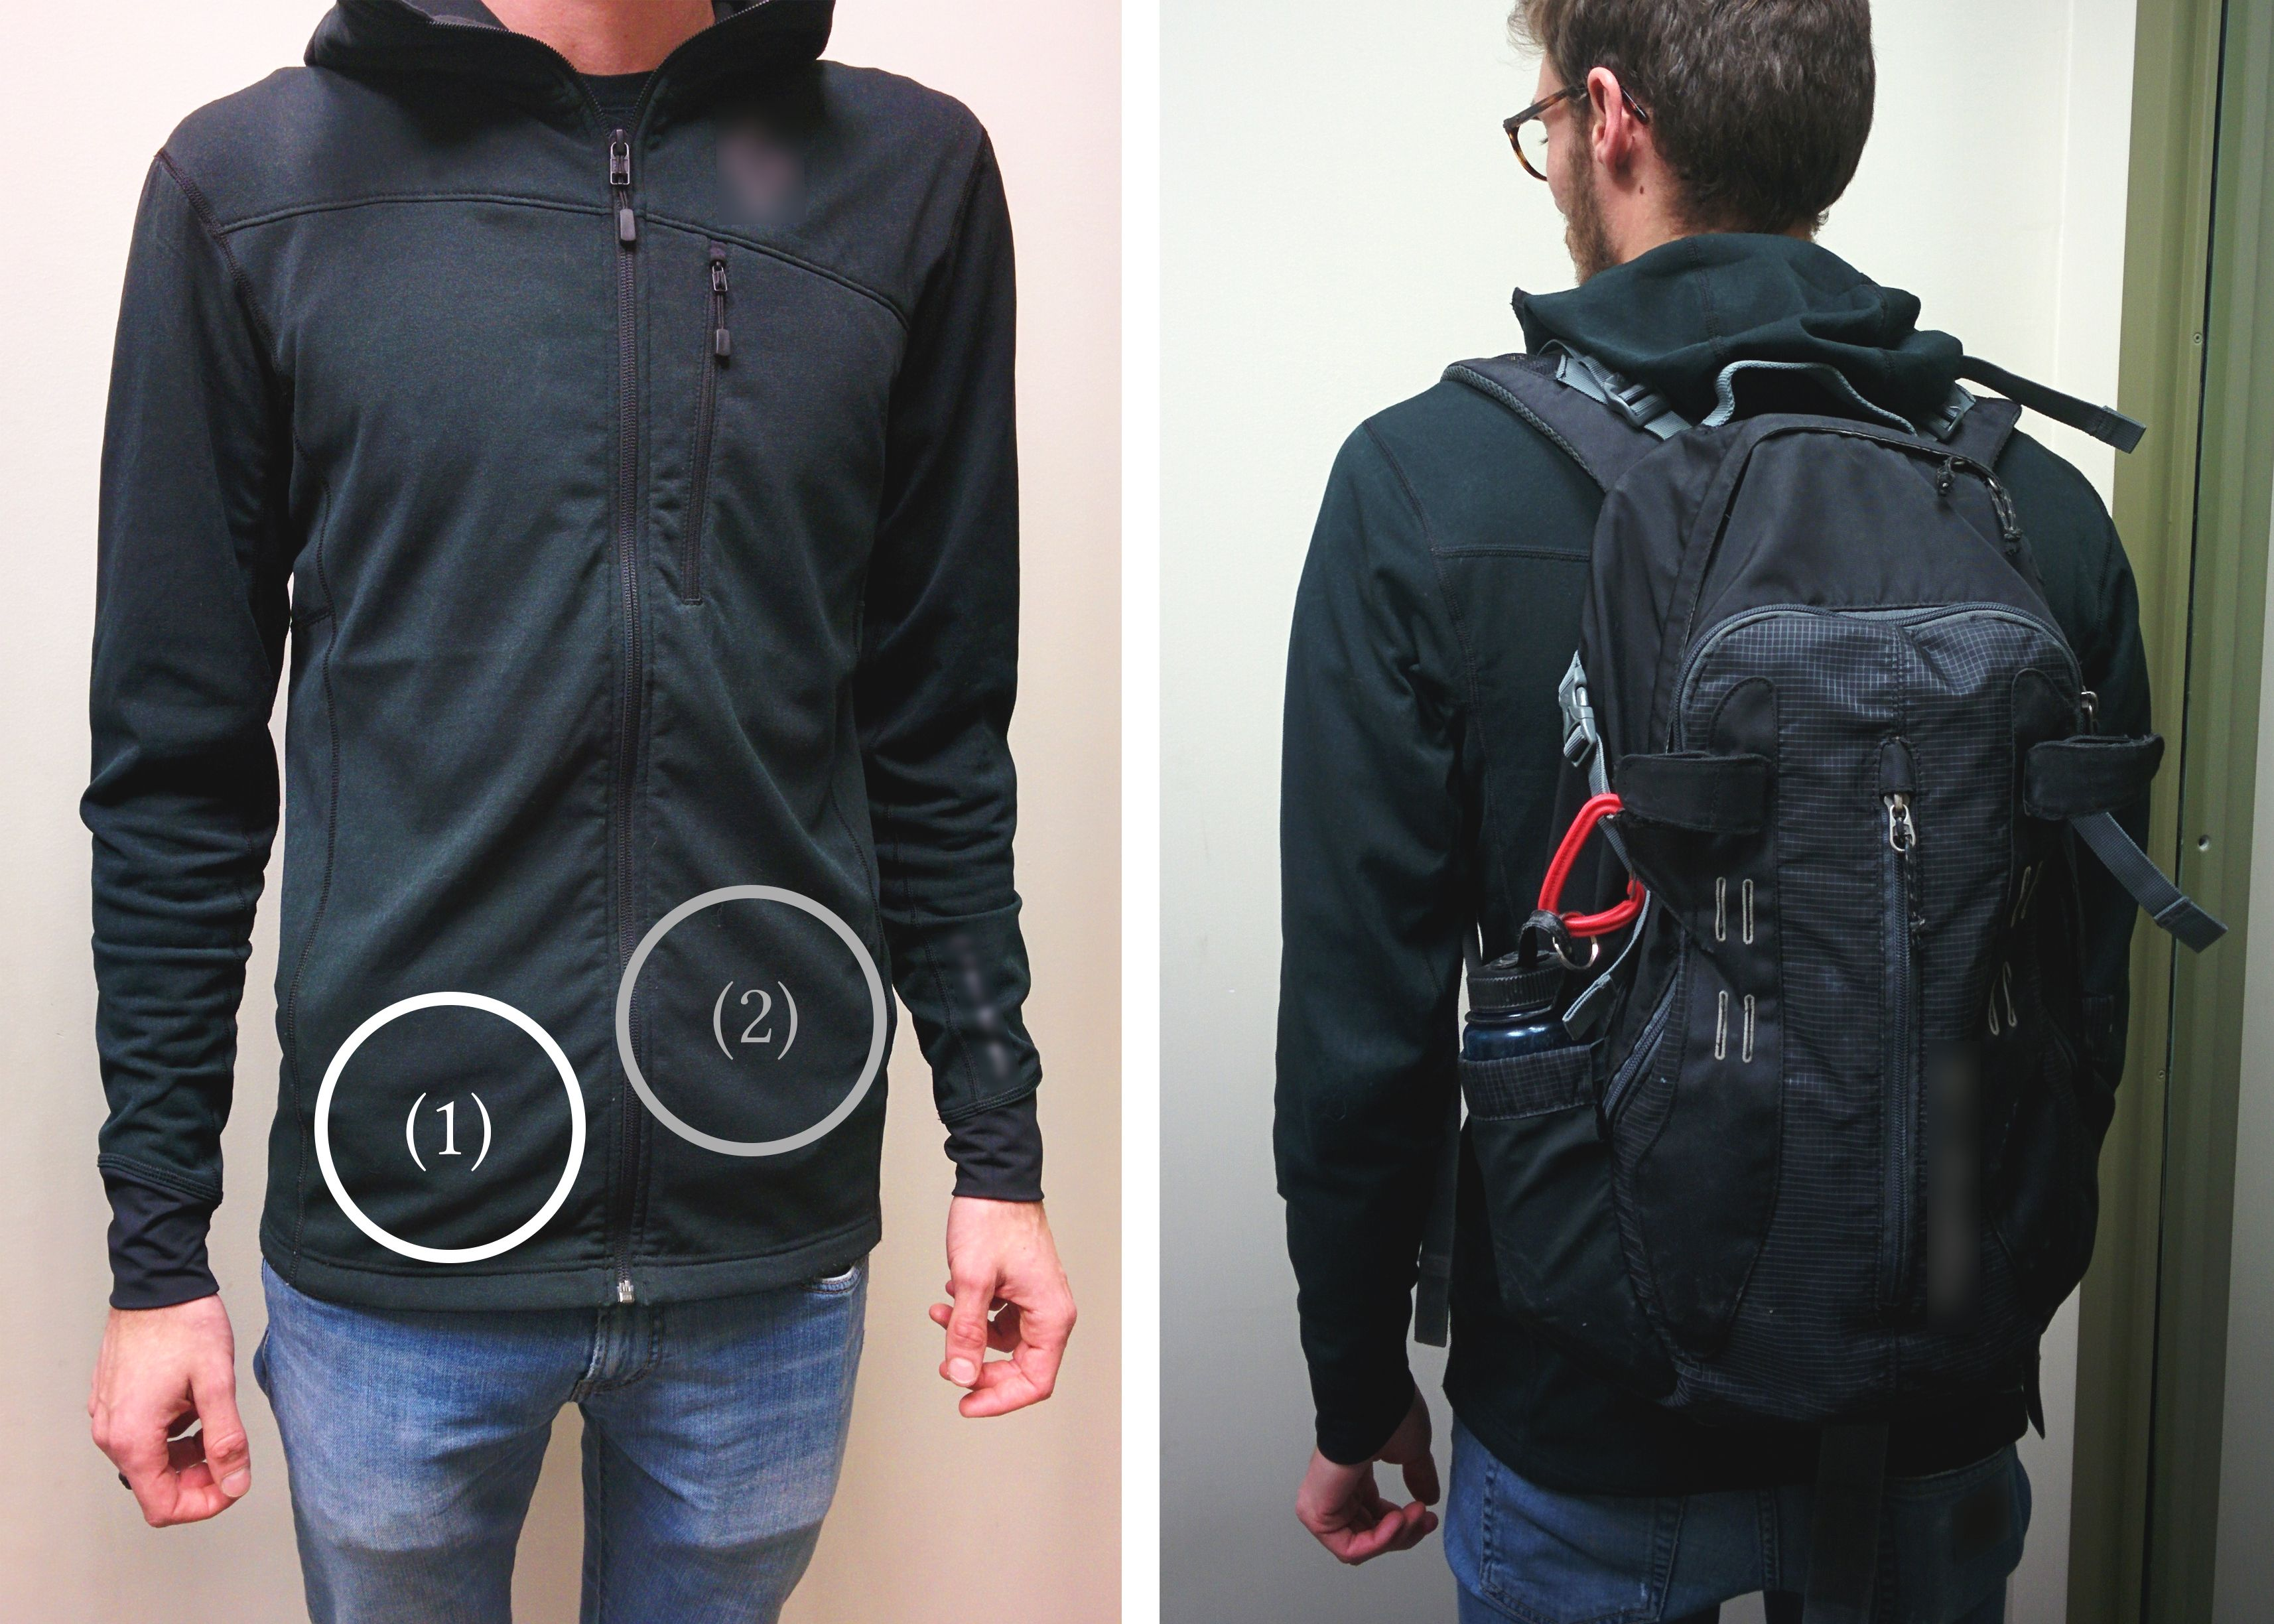
\includegraphics[width=2.8in]{positions.jpg}
%   \caption{From left to right, position of the wearable device inside both right (1) and left (2) front jacket pockets and inside a standard 20L backpack.}
%   \label{fig:positions}
% \end{figure}

Once participants were introduced how to wear both devices, % in the same indicated position and at the same time, 
they were invited to perform six round trips on each soil types, for each given position. % A supervisor, in charge of the management of the data record for both devices, let them know both when to start and stop walking. Firstly, they were asked to begin by gravels that were placed inside the box described previously. Secondly they were requested to perform the same operation on the floor next to the container that is considered to be a kind of cement. Finally, since we needed to replace gravels inside the container, participants were called back\textemdash at another stage\textemdash to perform the experiment once more, on the sand.

\section{Results}
% \subsection{Classification Performance Metrics}
% Since the performance of the classification task requires to be properly evaluated, it is important to provide representative metrics. 

% To this end, the accuracy ($Acc.$) is probably the most dominant measure in the literature because of its simplicity. This measure provides the ratio between the correct number of predictions and the total number of cases given as,

% \begin{equation}
% 	\label{eq:f_acc}
% 	Acc. = \frac{TP + TN}{TP + TN + FP + FN}
% \end{equation}

% \noindent where $TP$ and $TN$ refer to true positive and true negative predictions respectively, and the total additionally include false positive ($FP$) and false negative ($FN$) predictions.

% Despite its popularity, accuracy alone does typically not provide enough information to evaluate the robustness of prediction outcomes. Indeed, accuracy does not compensate for results that may be expected by luck. A high accuracy does not necessarily reflect an indicator of a high classification performance. This is the accuracy paradox. For instance, in a predictive classification setting, models with a given level of accuracy may have greater performances than models with higher accuracy. In that sense, as suggested by Ben-David \cite{Ben-David2007}, we decided to provide the Cohen\textquotesingle s kappa ($k$) evaluation metric as well. This measure takes into account such a paradox and remains a more relevant metric in classification evaluation such as the method we suggest in this paper. The kappa measure is given by,

% \begin{equation}
% 	\label{eq:kappa}
% 	k = \frac{P_o-P_e}{1-P_e}
% \end{equation}

% \noindent where $P_o$ and $P_e$ are the observed and the expected probabilities respectively. 

% Another well-known metrics which is often used in related literature and which we choose to provide additionally,  is the F-Score (F1),

% \begin{equation}
% 	\label{eq:f_score}
% 	F1 = 2\cdot\frac{Precision . Recall}{Precision + Recall}
% \end{equation}

% \noindent $Precision$ and $Recall$ are expressed by (\ref{eq:precision}) and (\ref{eq:recall}) respectively,

% \begin{equation}
% 	\label{eq:precision}
% 	Precision = \frac{TP}{TP + FP}
% \end{equation}

% \begin{equation}
% 	\label{eq:recall}
% 	Recall = \frac{TP}{TP + FN}
% \end{equation}

% \noindent where $FP$ and $FN$ refer to false positive and false negative predictions respectively and $TP$ corresponds to true positive results.

\subsection{Datasets}

Through the recorded raw data, several datasets have been produced. Details about each of them are provided in Table \ref{tab:datasets}. In the same way as our previous work {\cite{Thullier2017b}}, each dataset was split  in several subsets of $6 \times 60$ instances to obtain one sample per round trip. Thus, we obtained an average total of 5 samples for each participant, on each soil type, for each position of the device on which features were extracted for each device regrouped by the total number of axes.

% Once every participant has achieved the experiment on all soil types, we had to produce several datasets in order to make sure that the method we suggest in this paper was accurate and reliable enough. Details about each dataset are provided in Table \ref{tab:datasets}, and they were all made freely accessible to the public \cite{Thullier2017}. 

% As we have detailed in an above section, the data sampling provided by our two devices was made at a 60 Hz frequency. Moreover, we have observed an average time of 6 seconds for participants to complete a round trip both in the box, as well as outside the box on the cement. Hence, we have decided to split our dataset in several subsets of $6 \times 60$ instances in order to produce one sample per round trip. Thus, we obtained an average total of 5 samples, for each participant, on each soil type, for each position of the device on which features were extracted for each devices regrouped by the total number of axis. (\textit{i.e.} 6, 9, 12).

\begin{table}[!ht]
    \centering
    \caption{The detailed list of produced datasets where the name of each dataset is expressed with the BNF notation.}
    \label{tab:datasets}
    \resizebox{.8\columnwidth}{!} 
	{
   		\begin{tabular}{rl}
    		\toprule
        		\textbf{Dataset}
        		&\textbf{Description}\\
        	\midrule
    			\multirow{2}{*}{$\textbf{soil\_type\_}[\textbf{wear} | \textbf{cell}]\_[\textbf{6} | \textbf{9} | \textbf{12}]$}
    			&Instances are annotated\\&only with the related soil type. \\
    		\midrule
    			\multirow{3}{*}{$\textbf{soil\_type\_people\_}[\textbf{wear} | \textbf{cell}]\_[\textbf{6} | \textbf{9} | \textbf{12}]$}
    			&Instances are annotated both\\&with the related soil type and the \\&participant's letter.\\
    		\midrule  
    			\multirow{3}{*}{$\textbf{soil\_type\_position\_}[\textbf{wear} | \textbf{cell}]\_[\textbf{6} | \textbf{9} | \textbf{12}]$}
    			&Instances are annotated both\\&with the related soil type and the\\&location of the given device.\\
    		\bottomrule
    	\end{tabular}
    }
\end{table}

% As we have mentioned in the above section, only a smaller number of the same participants were available to achieve this new experiment and it was not possible to record data on the snow. In that sense, we took care of removing all the corresponding entries in each previously suggested dataset.

Since it is known that the human gait is considered to be a behavioral biometric \cite{Thullier2016c}, we have constructed one particular dataset containing each soil type for each participant for the most accurate acquisition technique. These 6 datasets let us experience the user-independent assumption. Moreover, since we have exploited several positions, a dataset per soil types was created to test the position-independent hypothesis. 

% Since it is known that the human gait is considered to be a behavioral biometric \cite{Thullier2016c}, we have constructed one particular dataset containing each soil type for each participant for the most accurate acquisition technique. Hence, these 6 datasets let us experiment the user-independent assumption of our method. Moreover, since we have exploited several positions for the wearable device, we have also created one dataset containing every soil types for each given place, being 5 distinct datasets in total. In that sense, we have been able to test the position-independent hypothesis as well. 

\subsection{Results Obtained}

The performance of the whole comparison provided here was evaluated through the same 10-folds cross validation method over the same parameter tuning for each classification algorithms that were employed in our previous work {\cite{Thullier2017b}}. As recall, when using the random forest algorithm, the parameters that were selected to perform the comparison were $B=150$ or $B=300$ trees and for each case, $F=\lfloor\frac{1}{2}\sqrt{m}\rfloor$, $F=\lfloor\log_2(m)+1\rfloor$ or $F=\lfloor\sqrt{m}\rfloor$ random variables. With the $k$-NN algorithm, these parameters where $k=1$ nearest neighbors as well as both the Euclidean and the Manhattan distance measure.

% The performance for the different methods of acquisition to recognize soil types through inertial data was compared according to several classification analyses. These assessments were achieved thanks to the \textit{WEKA} datamining software \cite{Hall2009} which was used as a library in a simple open-source \textit{Java} Command Line Interface (CLI) application \cite{Thullier2016a}. Through this program, a 10-folds cross validation method was employed to quantify each trained model that was constructed. 

% First of all, few Random Forest models were created based on the same parameters tuning suggested in our previous work \cite{Thullier2017b}. As Breiman \cite{Breiman2001} suggests that it is preferable to have a great number of trees in the forest, we have decided to keep from our previous work both $B = 150$ and $B = 300$ trees in order to preserve an acceptable computation time. Moreover, since the number of random variables ($F$) strongly depends on the number of features, this parameter must necessarily vary according to the number of axes ($m$). In that sense, we also conserve the comparison of the performance between the same three following values: $F=\lfloor\frac{1}{2}\sqrt{m}\rfloor$, $F=\lfloor\log_2(m)+1\rfloor$ and $F=\lfloor\sqrt{m}\rfloor$, where $m = 70$, $105$ and $140$ for a 6, 9 and 12-axis dataset, respectively. Finally, the default function used to measure the quality of the split which is implemented in \textit{WEKA} is the information gain.

% Similarly, the performance of the $k$-Nearest Neighbors algorithm was evaluated over all the proposed datasets, to compare the results obtained with the Random Forest algorithm. The two measures of distance described previously were experienced in this appraisal and based on our previous work, the fitting number of neighbors to consider stayed only one. Indeed, all values from $k=1$ to $k=\sqrt{m}$ were tested, for each value of $m$, depending on the number of axes. The results were compared in an empirical manner to find such an optimal setting.

\subsubsection{Wearable Device}
This section exposes the results obtained when using every set of features samples extracted from every acquisition method for the wearable device. Nevertheless, results of our previous work were modified to handle the loss of participants as well as our impossibility to perform any records on the snow. This paper only presents detailed results in Tables \ref{tab:wear_rf} and \ref{tab:wear_knn}, with the parameters tuning that let us obtain the best overall recognition rate for the two different classification algorithms. When using the wearable device, optimal parameters are either $B=300$ trees and a number of random variables equivalent to $F=\lfloor\log_2(m)+1\rfloor$, or $k = 1$ neighbor and a Manhattan distance measure for the RF and the $k$-NN classifier respectively.

% Tables \ref{tab:rf150_wear} and \ref{tab:rf300_wear} exposes the outcomes of the classification process when the RF algorithm was, tuned with both $B=150$ and $B=300$ trees, respectively.

\begin{table}[!ht]
	\centering
	\caption{Results of RF classification using $B=300$ trees and $F=\lfloor\log_2(m)+1\rfloor$ as parameters for the wearable.}
    \label{tab:wear_rf}
    \scalebox{0.75}
    {
        \begin{tabular}{rccc}
            \toprule
            	\textbf{Dataset}
            	&\textbf{Acc.}
            	&\textbf{F1}
            	&\textbf{k} \\
            \midrule
                soil\_type\_wear\_6             & 0.87 & 0.87 & 0.83 \\
                soil\_type\_wear\_9             & 0.92 & 0.92 & 0.88 \\
                soil\_type\_wear\_12            & 0.90 & 0.90 & 0.84 \\
                soil\_type\_people\_wear\_6     & 0.88 & 0.88 & 0.88 \\
                soil\_type\_people\_wear\_9     & 0.91 & 0.91 & \cellcolor{black!25}0.91 \\
                soil\_type\_people\_wear\_12    & 0.91 & 0.91 & 0.91 \\
                soil\_type\_position\_wear\_6   & 0.92 & 0.92 & 0.92 \\
                soil\_type\_position\_wear\_9   & 0.92 & 0.92 & \cellcolor{black!25}0.92 \\
                soil\_type\_position\_wear\_12  & 0.92 & 0.92 & 0.91 \\
            \bottomrule
        \end{tabular}
    }
\end{table}

\begin{table}[!ht]
	\centering
	\caption{Results of $k$-NN classification (where $k=1$), using the Manhattan distance for the wearable.}
	\label{tab:wear_knn}
	\scalebox{0.75}
	{
		\begin{tabular}{rccc}
			\toprule
			    \textbf{Dataset}
			    & \textbf{Acc.}
			    & \textbf{F1}
			    & \textbf{k} \\
			\midrule
			soil\_type\_wear\_6            & 0.92 & 0.92 & 0.90 \\
			soil\_type\_wear\_9            & 0.93 & 0.93 & 0.89 \\
			soil\_type\_wear\_12           & 0.90 & 0.90 & 0.85 \\
			soil\_type\_people\_wear\_6    & 0.89 & 0.89 & 0.89 \\
			soil\_type\_people\_wear\_9    & 0.92 & 0.92 & 0.91 \\
			soil\_type\_people\_wear\_12   & 0.90 & 0.90 & 0.89 \\
			soil\_type\_position\_wear\_6  & 0.87 & 0.87 & 0.86 \\
			soil\_type\_position\_wear\_9  & 0.91 & 0.91 & 0.91 \\
			soil\_type\_position\_wear\_12 & 0.87 & 0.87 & 0.86 \\
			\bottomrule
		\end{tabular}
	}
\end{table}

Through such results, a significant overall improvement with the upgraded version of the wearable device is noticeable. As an example, a rise of the median F-Score from 86\% with the 6-axis IMU to 92\% with the new 9-axis IMU has been observed when only considering soil type recognition. Moreover, it is possible to observe that the performance gains when including the Euler angles is almost negligible in every case.

% Through such results, a significant overall improvement with the upgraded version of the wearable device is noticeable. As an example, the median F-Score when only considering soil type recognition have risen from 86\% with the 6-axis IMU to 92\% with the new 9-axis IMU. Moreover, it is possible to observe that the performance gains when including the Euler angles is almost negligible in every case.

% \begin{table}[!ht]
% 	\centering
% 	\caption{Results of RF classification using $B=150$ trees and from up to down: $F=\lfloor\frac{1}{2}\sqrt{m}\rfloor$, $F=\lfloor\log_2(m)+1\rfloor$ and $F=\lfloor\sqrt{m}\rfloor$ as parameters for the wearable.}
% 	\label{tab:rf150_wear}
%     \scalebox{0.75}
% 	{
% 		\begin{tabular}{rccc}
% 			\toprule
% 			\textbf{Dataset}
% 			                               & \textbf{Acc.}
% 			                               & \textbf{F1}
% 			                               & \textbf{k}                  \\
% 			\midrule
% 			soil\_type\_wear\_6            & 0.86          & 0.86 & 0.82 \\
% 			soil\_type\_wear\_9            & 0.91          & 0.91 & 0.86 \\
% 			soil\_type\_wear\_12           & 0.89          & 0.89 & 0.83 \\
% 			soil\_type\_people\_wear\_6    & 0.88          & 0.88 & 0.88 \\
% 			soil\_type\_people\_wear\_9    & 0.91          & 0.91 & 0.90 \\
% 			soil\_type\_people\_wear\_12   & 0.92          & 0.92 & 0.91 \\
% 			soil\_type\_position\_wear\_6  & 0.91          & 0.90 & 0.90 \\
% 			soil\_type\_position\_wear\_9  & 0.93          & 0.93 & 0.92 \\
% 			soil\_type\_position\_wear\_12 & 0.92          & 0.92 & 0.91 \\
% 		\end{tabular}
% 	}
% 	\scalebox{0.75}
% 	{
% 		\begin{tabular}{rccc}
% 			% \toprule
% 			% \textbf{Dataset}
% 			% & \textbf{Acc.}
% 			% & \textbf{F1}
% 			% & \textbf{k} \\
% 			\midrule
% 			soil\_type\_wear\_6            & 0.86 & 0.86 & 0.81 \\
% 			soil\_type\_wear\_9            & 0.91 & 0.91 & 0.87 \\
% 			soil\_type\_wear\_12           & 0.89 & 0.89 & 0.83 \\
% 			soil\_type\_people\_wear\_6    & 0.88 & 0.88 & 0.87 \\
% 			soil\_type\_people\_wear\_9    & 0.91 & 0.91 & 0.91 \\
% 			soil\_type\_people\_wear\_12   & 0.91 & 0.91 & 0.91 \\
% 			soil\_type\_position\_wear\_6  & 0.91 & 0.91 & 0.91 \\
% 			soil\_type\_position\_wear\_9  & 0.92 & 0.92 & 0.91 \\
% 			soil\_type\_position\_wear\_12 & 0.92 & 0.92 & 0.92 \\
% 		\end{tabular}
% 	}
% 	\scalebox{0.75}
% 	{
% 		\begin{tabular}{rccc}
% 			% \toprule
% 			%     \textbf{Dataset}
% 			%     & \textbf{Acc.}
% 			%     & \textbf{F1}
% 			%     & \textbf{k} \\
% 			\midrule
% 			soil\_type\_wear\_6            & 0.86 & 0.86 & 0.81 \\
% 			soil\_type\_wear\_9            & 0.90 & 0.90 & 0.85 \\
% 			soil\_type\_wear\_12           & 0.90 & 0.90 & 0.85 \\
% 			soil\_type\_people\_wear\_6    & 0.86 & 0.86 & 0.85 \\
% 			soil\_type\_people\_wear\_9    & 0.91 & 0.91 & 0.91 \\
% 			soil\_type\_people\_wear\_12   & 0.91 & 0.91 & 0.90 \\
% 			soil\_type\_position\_wear\_6  & 0.91 & 0.91 & 0.90 \\
% 			soil\_type\_position\_wear\_9  & 0.92 & 0.92 & 0.91 \\
% 			soil\_type\_position\_wear\_12 & 0.91 & 0.91 & 0.91 \\
% 			\bottomrule
% 		\end{tabular}
% 	}
% \end{table}

% \begin{table}[!ht]
%     \centering
%     \caption{Results of RF classification using $B=300$ trees and from up to down: $F=\lfloor\frac{1}{2}\sqrt{m}\rfloor$, $F=\lfloor\log_2(m)+1\rfloor$ and $F=\lfloor\sqrt{m}\rfloor$ as parameters for the wearable.}
%     \label{tab:rf300_wear}
%     \scalebox{0.75}
%     {
%         \begin{tabular}{rccc}
%             \toprule
%                 \textbf{Dataset}
%                 &\textbf{Acc.}
%                 &\textbf{F1}
%                 &\textbf{k} \\
%             \midrule
%                 soil\_type\_wear\_6             & 0.86 & 0.86 & 0.82 \\
%                 soil\_type\_wear\_9             & 0.92 & 0.92 & 0.87 \\
%                 soil\_type\_wear\_12            & 0.90 & 0.90 & 0.85 \\
%                 soil\_type\_people\_wear\_6     & 0.88 & 0.88 & 0.88 \\
%                 soil\_type\_people\_wear\_9     & 0.92 & 0.92 & 0.91 \\
%                 soil\_type\_people\_wear\_12    & 0.92 & 0.92 & 0.92 \\
%                 soil\_type\_position\_wear\_6   & 0.92 & 0.92 & 0.91 \\
%                 soil\_type\_position\_wear\_9   & 0.93 & 0.93 & 0.91 \\
%                 soil\_type\_position\_wear\_12  & 0.92 & 0.92 & 0.91 \\
%         \end{tabular}
%     }
%     \scalebox{0.75}
%     {
%         \begin{tabular}{rccc}
%             % \toprule
%             % 	\textbf{Dataset}
%             % 	&\textbf{Acc.}
%             % 	&\textbf{F1}
%             % 	&\textbf{k} \\
%             \midrule
%                 soil\_type\_wear\_6             & 0.87 & 0.87 & 0.83 \\
%                 soil\_type\_wear\_9             & 0.92 & 0.92 & 0.88 \\
%                 soil\_type\_wear\_12            & 0.90 & 0.90 & 0.84 \\
%                 soil\_type\_people\_wear\_6     & 0.88 & 0.88 & 0.88 \\
%                 soil\_type\_people\_wear\_9     & 0.91 & 0.91 & \cellcolor{black!25}0.91 \\
%                 soil\_type\_people\_wear\_12    & 0.91 & 0.91 & 0.91 \\
%                 soil\_type\_position\_wear\_6   & 0.92 & 0.92 & 0.92 \\
%                 soil\_type\_position\_wear\_9   & 0.92 & 0.92 & \cellcolor{black!25}0.92 \\
%                 soil\_type\_position\_wear\_12  & 0.92 & 0.92 & 0.91 \\
%         \end{tabular}
%     }
%     \scalebox{0.75}
%     {
%         \begin{tabular}{rccc}
%             % \toprule
%             %     \textbf{Dataset}
%             %     &\textbf{Acc.}
%             %     &\textbf{F1}
%             %     &\textbf{k} \\
%             \midrule  	
%                 soil\_type\_wear\_6             & 0.86 & 0.86 & 0.82 \\
%                 soil\_type\_wear\_9             & 0.92 & 0.92 & 0.87 \\
%                 soil\_type\_wear\_12            & 0.91 & 0.91 & 0.86 \\
%                 soil\_type\_people\_wear\_6     & 0.87 & 0.87 & 0.86 \\
%                 soil\_type\_people\_wear\_9     & 0.91 & 0.91 & 0.87 \\
%                 soil\_type\_people\_wear\_12    & 0.91 & 0.91 & 0.91 \\
%                 soil\_type\_position\_wear\_6   & 0.92 & 0.92 & 0.92 \\
%                 soil\_type\_position\_wear\_9   & 0.92 & 0.92 & 0.92 \\
%                 soil\_type\_position\_wear\_12  & 0.92 & 0.92 & 0.92 \\ 	
%             \bottomrule
%         \end{tabular}
%     }
% \end{table}

% Based on our previous work {\cite{Thullier2017b}}, the performance of the RF classifier must also be compared with a classification with the $k$-NN algorithm. Table \ref{tab:knn_wear} provides the outcomes for both the Euclidean and the Manhattan measures respectively. In the same way as the results we obtained beforehand, the performance, with the two distance measures, was mostly analog to the ones that were achieved with the various parameters tuning of the RF algorithm. However, slightly superior results with the Manhattan distance measure comparatively to the Euclidean one were noticeable as well.

% \begin{table}[!ht]
%     \centering
%     \caption{Results of $k$-NN classification (where $k=1$), using from up to down: the Euclidean and the Manhattan distance for the wearable.}
%     \label{tab:knn_wear}
%     \scalebox{0.75}
%     {
%         \begin{tabular}{rccc}
%             \toprule
%                 \textbf{Dataset}
%                 & \textbf{Acc.}
%                 & \textbf{F1}
%                 & \textbf{k} \\
%             \midrule
%                 soil\_type\_wear\_6            & 0.91 & 0.91 & 0.87 \\
%                 soil\_type\_wear\_9            & 0.90 & 0.90 & 0.85 \\
%                 soil\_type\_wear\_12           & 0.84 & 0.84 & 0.76 \\
%                 soil\_type\_people\_wear\_6    & 0.87 & 0.88 & 0.87 \\
%                 soil\_type\_people\_wear\_9    & 0.90 & 0.90 & 0.89 \\
%                 soil\_type\_people\_wear\_12   & 0.87 & 0.87 & 0.86 \\
%                 soil\_type\_position\_wear\_6  & 0.84 & 0.84 & 0.83 \\
%                 soil\_type\_position\_wear\_9  & 0.88 & 0.88 & 0.88 \\
%                 soil\_type\_position\_wear\_12 & 0.83 & 0.83 & 0.82 \\
%         \end{tabular}
%     }
%     \scalebox{0.75}
%     {
%         \begin{tabular}{rccc}
%             % \toprule
%             %     \textbf{Dataset}
%             %     & \textbf{Acc.}
%             %     & \textbf{F1}
%             %     & \textbf{k} \\
%             \midrule
%                 soil\_type\_wear\_6            & 0.92 & 0.92 & 0.90 \\
%                 soil\_type\_wear\_9            & 0.93 & 0.93 & 0.89 \\
%                 soil\_type\_wear\_12           & 0.90 & 0.90 & 0.85 \\
%                 soil\_type\_people\_wear\_6    & 0.89 & 0.89 & 0.89 \\
%                 soil\_type\_people\_wear\_9    & 0.92 & 0.92 & 0.91 \\
%                 soil\_type\_people\_wear\_12   & 0.90 & 0.90 & 0.89 \\
%                 soil\_type\_position\_wear\_6  & 0.87 & 0.87 & 0.86 \\
%                 soil\_type\_position\_wear\_9  & 0.91 & 0.91 & 0.91 \\
%                 soil\_type\_position\_wear\_12 & 0.87 & 0.87 & 0.86 \\
%             \bottomrule
%         \end{tabular}
%     }
% \end{table}

% As regards these overall results obtained with all the data produced by the wearable device, the recommendations concerning parameters that must be applied for the two classifiers that have been expressed in our previous work remains identical. Through these news findings, we can state that using either a Random Forest classifier with $B=300$ trees and a number of random variables equivalent to $F=\lfloor\log_2(m)+1\rfloor$, or a $k$-Nearest Neighbors classifier with $k = 1$ neighbor and a Manhattan distance measure, should outperform every other recognition configurations.

\subsubsection{Mobile Device}
In the same way as for the wearable device, this section only exposes, in Table \ref{tab:cell_rf} and \ref{tab:cell_knn}, results obtained when using optimal parameters for both classification techniques when applied on every set of features samples extracted from every acquisition method for the mobile device.

\begin{table}[!ht]
	\centering
	\caption{Results of RF classification using $B=300$ trees and $F=\lfloor\log_2(m)+1\rfloor$ as parameters for the mobile.}
	\label{tab:cell_rf}
	\scalebox{0.75}
	{
		\begin{tabular}{rccc}
			\toprule
			    \textbf{Dataset}
			    & \textbf{Acc.}
			    & \textbf{F1}
			    & \textbf{k} \\
			\midrule
                soil\_type\_cell\_6            & 0.92 & 0.92 & 0.88                     \\
                soil\_type\_cell\_9            & 0.92 & 0.92 & 0.88                     \\
                soil\_type\_cell\_12           & 0.92 & 0.92 & 0.87                     \\
                soil\_type\_people\_cell\_6    & 0.91 & 0.91 & 0.91                     \\
                soil\_type\_people\_cell\_9    & 0.92 & 0.92 & \cellcolor{black!25}0.91 \\
                soil\_type\_people\_cell\_12   & 0.91 & 0.91 & 0.91                     \\
                soil\_type\_position\_cell\_6  & 0.92 & 0.92 & 0.91                     \\
                soil\_type\_position\_cell\_9  & 0.92 & 0.92 & \cellcolor{black!25}0.92 \\
                soil\_type\_position\_cell\_12 & 0.92 & 0.92 & 0.91                     \\
            \bottomrule
		\end{tabular}
	}
\end{table}

\begin{table}[!ht]
	\centering
	\caption{Results of $k$-NN classification (where $k=1$), using the Manhattan distance for the mobile.}
	\label{tab:cell_knn}
	\scalebox{0.75}
	{
		\begin{tabular}{rccc}
			\toprule
			    \textbf{Dataset}
			    & \textbf{Acc.}
			    & \textbf{F1}
			    & \textbf{k} \\
			\midrule
                soil\_type\_cell\_6            & 0.92 & 0.92 & 0.87 \\
                soil\_type\_cell\_9            & 0.92 & 0.92 & 0.87 \\
                soil\_type\_cell\_12           & 0.92 & 0.92 & 0.89 \\
                soil\_type\_people\_cell\_6    & 0.89 & 0.89 & 0.89 \\
                soil\_type\_people\_cell\_9    & 0.90 & 0.90 & 0.89 \\
                soil\_type\_people\_cell\_12   & 0.89 & 0.89 & 0.89 \\
                soil\_type\_position\_cell\_6  & 0.90 & 0.90 & 0.89 \\
                soil\_type\_position\_cell\_9  & 0.89 & 0.89 & 0.88 \\
                soil\_type\_position\_cell\_12 & 0.91 & 0.91 & 0.90 \\
			\bottomrule
		\end{tabular}
	}
\end{table}

% every set of features samples extracted from every acquisition method for a mobile device. Tables \ref{tab:rf150_cell} and \ref{tab:rf300_cell} exposes the outcomes of the classification process when the RF algorithm was, tuned with both $B=150$ and $B=300$ trees, respectively. In the same way, Table \ref{tab:knn_cell} provides the results for the $k$-NN classification when setup with both the Euclidean and the Manhattan measures.

% \begin{table}[!ht]
%     \centering
%     \caption{Results of RF classification using $B=150$ trees and from up to down: $F=\lfloor\frac{1}{2}\sqrt{m}\rfloor$, $F=\lfloor\log_2(m)+1\rfloor$ and $F=\lfloor\sqrt{m}\rfloor$ as parameters for the mobile.}
%     \label{tab:rf150_cell}
%     \scalebox{0.75}
%     {
%         \begin{tabular}{rccc}
%             \toprule
%                 \textbf{Dataset}
%                 & \textbf{Acc.}
%                 & \textbf{F1}
%                 & \textbf{k} \\
%             \midrule
%                 soil\_type\_cell\_6            & 0.92 & 0.92 & 0.87 \\
%                 soil\_type\_cell\_9            & 0.92 & 0.92 & 0.88 \\
%                 soil\_type\_cell\_12           & 0.91 & 0.91 & 0.87 \\
%                 soil\_type\_people\_cell\_6    & 0.91 & 0.91 & 0.90 \\
%                 soil\_type\_people\_cell\_9    & 0.91 & 0.91 & 0.91 \\
%                 soil\_type\_people\_cell\_12   & 0.91 & 0.91 & 0.91 \\
%                 soil\_type\_position\_cell\_6  & 0.91 & 0.91 & 0.91 \\
%                 soil\_type\_position\_cell\_9  & 0.91 & 0.91 & 0.91 \\
%                 soil\_type\_position\_cell\_12 & 0.92 & 0.92 & 0.91 \\
%         \end{tabular}
%     }
%     \scalebox{0.75}
%     {
%         \begin{tabular}{rccc}
%             % \toprule
%                 % \textbf{Dataset}
%                 % & \textbf{Acc.}
%                 % & \textbf{F1}
%                 % & \textbf{k} \\
%             \midrule
%                 soil\_type\_cell\_6            & 0.92 & 0.92 & 0.88 \\
%                 soil\_type\_cell\_9            & 0.92 & 0.92 & 0.88 \\
%                 soil\_type\_cell\_12           & 0.92 & 0.92 & 0.88 \\
%                 soil\_type\_people\_cell\_6    & 0.91 & 0.91 & 0.91 \\
%                 soil\_type\_people\_cell\_9    & 0.92 & 0.92 & 0.91 \\
%                 soil\_type\_people\_cell\_12   & 0.91 & 0.91 & 0.91 \\
%                 soil\_type\_position\_cell\_6  & 0.92 & 0.92 & 0.91 \\
%                 soil\_type\_position\_cell\_9  & 0.92 & 0.92 & 0.91 \\
%                 soil\_type\_position\_cell\_12 & 0.92 & 0.92 & 0.92 \\
%         \end{tabular}
%     }
%     \scalebox{0.75}
%     {
%         \begin{tabular}{rccc}
%             % \toprule
%             %     \textbf{Dataset}
%             %     & \textbf{Acc.}
%             %     & \textbf{F1}
%             %     & \textbf{k} \\
%             \midrule
%                 soil\_type\_cell\_6            & 0.92 & 0.92 & 0.89 \\
%                 soil\_type\_cell\_9            & 0.91 & 0.91 & 0.87 \\
%                 soil\_type\_cell\_12           & 0.92 & 0.92 & 0.88 \\
%                 soil\_type\_people\_cell\_6    & 0.91 & 0.91 & 0.90 \\
%                 soil\_type\_people\_cell\_9    & 0.92 & 0.92 & 0.91 \\
%                 soil\_type\_people\_cell\_12   & 0.91 & 0.91 & 0.91 \\
%                 soil\_type\_position\_cell\_6  & 0.92 & 0.92 & 0.91 \\
%                 soil\_type\_position\_cell\_9  & 0.92 & 0.92 & 0.91 \\
%                 soil\_type\_position\_cell\_12 & 0.92 & 0.92 & 0.92 \\
%             \bottomrule
%         \end{tabular}
%     }
% \end{table}

% \begin{table}[!ht]
%     \centering
%     \caption{Results of RF classification using $B=300$ trees and from up to down: $F=\lfloor\frac{1}{2}\sqrt{m}\rfloor$, $F=\lfloor\log_2(m)+1\rfloor$ and $F=\lfloor\sqrt{m}\rfloor$ as parameters for the mobile.}
%     \label{tab:rf300_cell}
%     \scalebox{0.75}
%     {
%         \begin{tabular}{rccc}
%             \toprule
%                 \textbf{Dataset}
%                 & \textbf{Acc.}
%                 & \textbf{F1}
%                 & \textbf{k} \\
%             \midrule
%                 soil\_type\_cell\_6            & 0.92 & 0.92 & 0.88 \\
%                 soil\_type\_cell\_9            & 0.92 & 0.92 & 0.88 \\
%                 soil\_type\_cell\_12           & 0.92 & 0.92 & 0.88 \\
%                 soil\_type\_people\_cell\_6    & 0.91 & 0.91 & 0.91 \\
%                 soil\_type\_people\_cell\_9    & 0.91 & 0.91 & 0.91 \\
%                 soil\_type\_people\_cell\_12   & 0.91 & 0.91 & 0.91 \\
%                 soil\_type\_position\_cell\_6  & 0.92 & 0.92 & 0.91 \\
%                 soil\_type\_position\_cell\_9  & 0.92 & 0.92 & 0.92 \\
%                 soil\_type\_position\_cell\_12 & 0.92 & 0.92 & 0.91 \\
%         \end{tabular}
%     }
%     \scalebox{0.75}
%     {
%         \begin{tabular}{rccc}
%             % \toprule
%             %     \textbf{Dataset}
%             %     & \textbf{Acc.}
%             %     & \textbf{F1}
%             %     & \textbf{k} \\
%             \midrule
%                 soil\_type\_cell\_6            & 0.92 & 0.92 & 0.88                     \\
%                 soil\_type\_cell\_9            & 0.92 & 0.92 & 0.88                     \\
%                 soil\_type\_cell\_12           & 0.92 & 0.92 & 0.87                     \\
%                 soil\_type\_people\_cell\_6    & 0.91 & 0.91 & 0.91                     \\
%                 soil\_type\_people\_cell\_9    & 0.92 & 0.92 & \cellcolor{black!25}0.91 \\
%                 soil\_type\_people\_cell\_12   & 0.91 & 0.91 & 0.91                     \\
%                 soil\_type\_position\_cell\_6  & 0.92 & 0.92 & 0.91                     \\
%                 soil\_type\_position\_cell\_9  & 0.92 & 0.92 & \cellcolor{black!25}0.92 \\
%                 soil\_type\_position\_cell\_12 & 0.92 & 0.92 & 0.91                     \\
%         \end{tabular}
%     }
%     \scalebox{0.75}
%     {
%         \begin{tabular}{rccc}
%             % \toprule
%             %     \textbf{Dataset}
%             %     & \textbf{Acc.}
%             %     & \textbf{F1}
%             %     & \textbf{k} \\
%             \midrule
%                 soil\_type\_cell\_6            & 0.93 & 0.93 & 0.89 \\
%                 soil\_type\_cell\_9            & 0.92 & 0.92 & 0.88 \\
%                 soil\_type\_cell\_12           & 0.92 & 0.92 & 0.88 \\
%                 soil\_type\_people\_cell\_6    & 0.91 & 0.91 & 0.90 \\
%                 soil\_type\_people\_cell\_9    & 0.91 & 0.91 & 0.91 \\
%                 soil\_type\_people\_cell\_12   & 0.91 & 0.91 & 0.91 \\
%                 soil\_type\_position\_cell\_6  & 0.92 & 0.92 & 0.91 \\
%                 soil\_type\_position\_cell\_9  & 0.92 & 0.92 & 0.91 \\
%                 soil\_type\_position\_cell\_12 & 0.92 & 0.92 & 0.91 \\
%             \bottomrule
%         \end{tabular}
%     }
% \end{table}

% \begin{table}[!ht]
%     \centering
%     \caption{Results of $k$-NN classification (where $k=1$), using from up to down: the Euclidean and the Manhattan distance for the mobile.}
%     \label{tab:knn_cell}
%     \scalebox{0.75}
%     {
%         \begin{tabular}{rccc}
%             \toprule
%                 \textbf{Dataset}
%                 & \textbf{Acc.}
%                 & \textbf{F1}
%                 & \textbf{k} \\
%             \midrule
%                 soil\_type\_cell\_6            & 0.90 & 0.90 & 0.85 \\
%                 soil\_type\_cell\_9            & 0.90 & 0.90 & 0.85 \\
%                 soil\_type\_cell\_12           & 0.90 & 0.90 & 0.85 \\
%                 soil\_type\_people\_cell\_6    & 0.89 & 0.89 & 0.88 \\
%                 soil\_type\_people\_cell\_9    & 0.87 & 0.87 & 0.86 \\
%                 soil\_type\_people\_cell\_12   & 0.87 & 0.87 & 0.86 \\
%                 soil\_type\_position\_cell\_6  & 0.89 & 0.89 & 0.88 \\
%                 soil\_type\_position\_cell\_9  & 0.88 & 0.88 & 0.87 \\
%                 soil\_type\_position\_cell\_12 & 0.89 & 0.89 & 0.88 \\
%         \end{tabular}
%     }
%     \scalebox{0.75}
%     {
%         \begin{tabular}{rccc}
%             % \toprule
%             %     \textbf{Dataset}
%             %     & \textbf{Acc.}
%             %     & \textbf{F1}
%             %     & \textbf{k} \\
%             \midrule
%                 soil\_type\_cell\_6            & 0.92 & 0.92 & 0.87 \\
%                 soil\_type\_cell\_9            & 0.92 & 0.92 & 0.87 \\
%                 soil\_type\_cell\_12           & 0.92 & 0.92 & 0.89 \\
%                 soil\_type\_people\_cell\_6    & 0.89 & 0.89 & 0.89 \\
%                 soil\_type\_people\_cell\_9    & 0.90 & 0.90 & 0.89 \\
%                 soil\_type\_people\_cell\_12   & 0.89 & 0.89 & 0.89 \\
%                 soil\_type\_position\_cell\_6  & 0.90 & 0.90 & 0.89 \\
%                 soil\_type\_position\_cell\_9  & 0.89 & 0.89 & 0.88 \\
%                 soil\_type\_position\_cell\_12 & 0.91 & 0.91 & 0.90 \\
%             \bottomrule
%         \end{tabular}
%     }
% \end{table}

These results demonstrate an excellent overall performance, for every dataset. Moreover, we observed that neither the acquisition method employed, nor the parameters tuning of the algorithms has affected the recognition rate since it stands truly similar in every case. Although the results appear to be slightly better than the ones obtained with the wearable devices, they remain mostly comparable. % particularly for both the 9 and 12-axis data records. The major difference with our wearable device is a greater recognition rate observed with 6-axis data produced by the mobile phone for every configurations.

% Finally, in regards to these new findings, we also recommend the same parameter configuration for both the two compared classification algorithms when applied on data recorded with a mobile phone.

\subsection{Independence Hypothesis}

Since our previous research have stated that the proposed soil types recognition method was position-independent, it is important to verify such a claim through these new results yet again. Results are shown in Figures \ref{fig:pi_wear} and \ref{fig:pi_cell}. The evaluation metric used as the position-independent baseline is the kappa measure being 92\% for both devices, as highlighted in Tables \ref{tab:wear_rf} and \ref{tab:cell_rf}. Although preceding overall results were indeed accurate, it is possible to observe an excellent performance, for both devices, when the learning process is achieved separately for each position as it was in our previous work. Moreover, there is no specific position that is greater than the baseline value in any cases.

% Since our previous research have stated that the proposed soil types recognition method was position-independent, it is important to verify such a claim through these new results yet again. To this end, we reproduced the same procedure, for the 9-axis acquisition method that is the more accurate, based on our previous observations. Hence, one dataset by position was created for each device and the evaluation was performed in the same manner, using parameters we recommended for the Random Forest algorithm (\textit{i.e.} $B=300$ trees and $F=\lfloor\log_2(m)+1\rfloor$). Results are shown in Figures \ref{fig:pi_wear} and \ref{fig:pi_cell}. The evaluation metric used as the position-independent baseline is the kappa measure being 92\% for both devices, as highlighted in tables \ref{tab:rf300_wear} and \ref{tab:rf300_cell}. Although preceding overall results were indeed accurate, it is possible to observe an excellent performance, for both devices, when the learning process is achieved separately for each position as it was in our previous work. Moreover, for both devices, there is no specific position that is greater than the baseline value.

\begin{figure}[!ht]
  \centering
  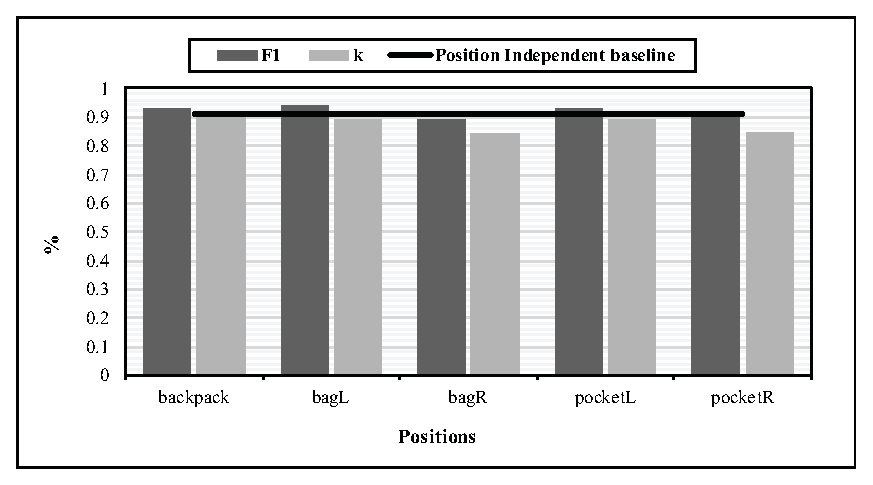
\includegraphics[width=2.4in]{pi_wear.eps}
  \caption{Kappa and F-Score measures comparison for both dependent and independent positions with the wearable device.}
  \label{fig:pi_wear}
\end{figure}

\begin{figure}[!ht]
  \centering
  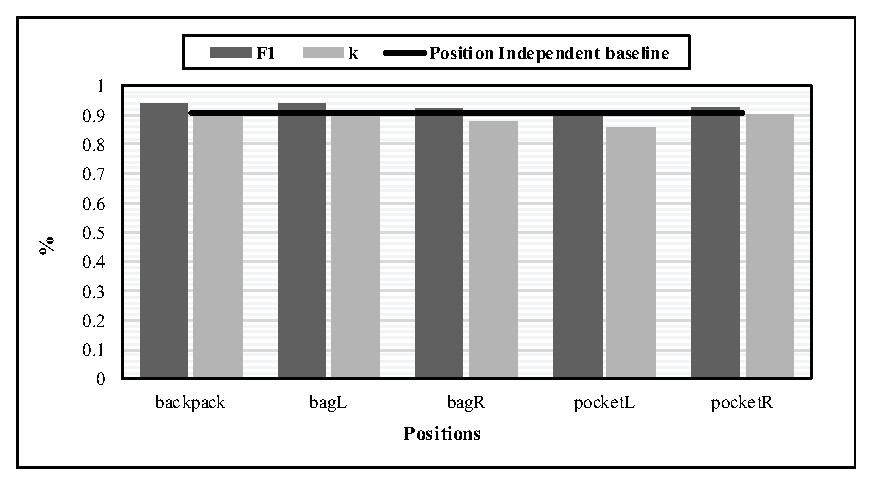
\includegraphics[width=2.4in]{pi_cell.eps}
  \caption{Kappa and F-Score measures comparison for both dependent and independent positions with the mobile device.}
  \label{fig:pi_cell}
\end{figure}

Additionally, the user-independent hypothesis was also verified based on our new results. In the same way as the position-independent assessment, one dataset by participants were generated and annotated with the corresponding soil type for the same acquisition method and for each device. Figures \ref{fig:ui_wear} and \ref{fig:ui_cell} show the obtained results, where the first chart refers to the wearable device analysis and the second corresponds to the mobile phone one. Both of them were computed with the same parameters as the position-independence verification. 

\begin{figure}[!ht]
	\centering
	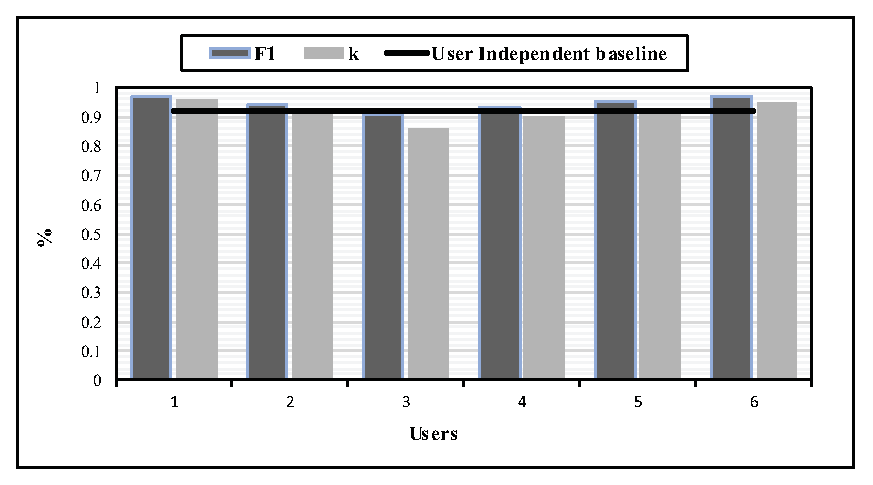
\includegraphics[width=2.4in]{ui_wear.eps}
	\caption{Kappa and F-Score measures comparison for both dependent and independent users with the wearable device, where each letter refers to a given participant.}
	\label{fig:ui_wear}
\end{figure}

\begin{figure}[!ht]
	\centering
	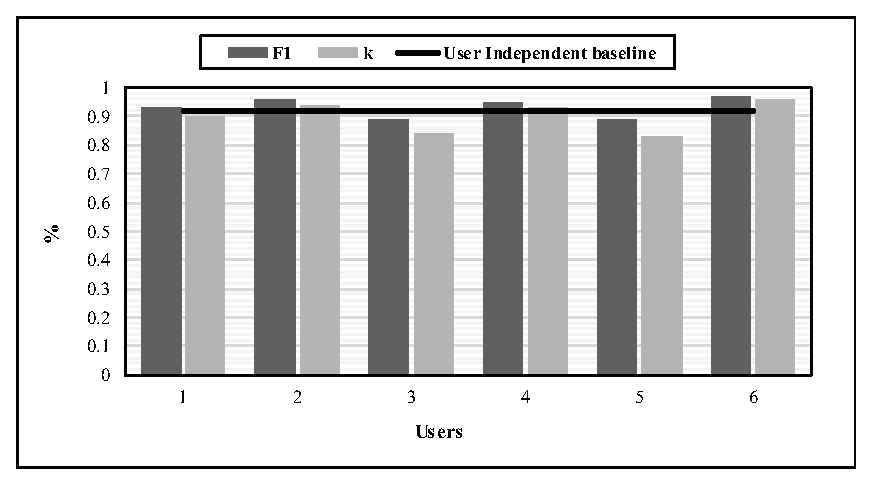
\includegraphics[width=2.4in]{ui_cell.eps}
	\caption{Kappa and F-Score measures comparison for both dependent and independent users with the mobile device, where each letter refers to a given participant.}
	\label{fig:ui_cell}
\end{figure}

Yet again, when compared to results that were achieved for the position-independence, the performance remains excellent when learning each participant individually for both devices. However, unlike the position-independence appraisal, there are few of given sets where the kappa measure exceeds the baseline value (\textit{i.e.} 91\% for both devices). In our previous research we have stated that due to a few number of participants, the user-independence condition was not possible to be acknowledged accurately. This new evaluation strengthens this belief since the number of involved participants is even smaller.

% Additionally, the user-independent hypothesis was also verified based on our new results. In the same way as the position-independent assessment, one dataset by participant were generated and annotated with the corresponding soil type for the same acquisition method (\textit{i.e.} 9-axis) and for each device. Figures \ref{fig:ui_wear} and \ref{fig:ui_cell} expose the obtained results, where the first chart refers to the wearable device analysis and the second corresponds to the mobile phone one. Both of them were computed with the same parameters as the position-independence verification. Yet again, when compared to results that were achieved for the position-independence, the performance remains excellent when learning each participant individually for both devices. However, unlike the position-independence appraisal, there are few of given sets where the kappa measure exceeds the baseline value (\textit{i.e.} 91\% for both devices). In our previous research we have stated that due to a too small number of participant, the user-independence condition was not possible to be acknowledged accurately. This new evaluation strengthens this belief since the number of involved participants is even smaller than before.

\section{Discussion}

According to the results detailed in the previous section, it is possible for us to say that the upgraded version of our device has enhanced the results we obtained before. When it was a matter of classifying only soil types, the accuracy has increased from 87\% to 92\%, in the best case, using respectively 6 and 9-axis data from the wearable device. However, when considering the additional time required by the processing of the Euler angles and the negligible performance gains they offer\textemdash we can state that preserving only 9-axis data records will be sufficient to achieve a suitable and accurate recognition of soil types.

Then, through the comparison of our wearable device with a mobile phone, a slight gap on the overall performances between both devices only when considering a 6-axis acquisition method was noticed. Such a difference could be explained first, by a poor quality of the 6-axis IMU embedded in the \textit{Arduino 101} board comparatively to the new \textit{LSM9DS1}. The other hypothesis refers to a prior filtering of data generated by the inertial sensor of the mobile device that undoubtedly make these data less noisy.

Finally, as regards the position-independence, it is possible for us to affirm that both the wearable device and the mobile phone will truly recognize the current soil type, no matter where they are worn by the user. However, just as our previous work, the even smaller number of users that it was possible to recruit do not allow us to acknowledge the user-independence accurately.

% In this research, we have compared our previously suggested method to recognize soil types through inertial data produced by a wearable device \cite{Thullier2017b}\textemdash first, with another inertial sensor providing more axes\textemdash as well as with a mobile devices that embedded a 9-axis IMU. According to the results detailed in the previous section, it is possible for us to say that the upgraded version of our device has enhanced the results we obtained before. The accuracy when it was a matter of classifying only soil types, have, in best case, increased from 87\% to 92\% using respectively 6 and 9-axis data from the wearable device. However when considering the additional time required by the processing of the Euler angles and the negligible performance gains they offer\textemdash it is possible for us to state that preserving only 9-axis data records will be sufficient to achieve a suitable and accurate recognition of soil types. 

% Then, through the comparison of our wearable device with a mobile phone, a gap on the overall performances between both devices only when considering a 6-axis acquisition method was exposed. Indeed, we showed that results obtained with the phone remain very stable no matter which acquisition method or algorithm was employed, whereas it is not the case for the wearable device. Such a difference could be explained first, by a poor quality of the 6-axis IMU embedded in the \textit{Arduino 101} board comparatively to the new \textit{LSM9DS1} inertial sensor. The other hypothesis refers to a prior filtering of data generated by the inertial sensor of the mobile device that undoubtedly make these data less noisy than the ones we recorded with our wearable device. Through this last assumption, no matter how accurate the results obtained with our wearable device are, we are confident that they may be improved yet. Insofar as it is known that inertial data are strongly sensitive to noise, we believe that applying a filter such as a low pass Finite Impulse Response (FIR) over raw inertial data should refine their quality. Moreover, few features within the ones that were extracted from the raw signal may not be discriminating enough and could, therefore, be removed to reduce the dimension of our datasets. These two possibilities of enhancement may undoubtedly result in a most valuable soil-types-recognition performance.

% Finally, the same conclusions as the ones we already drawn in our previous research may be extracted from both the position and the user independence conditions. The evaluation we have conducted to verify these two assumptions with our new sets of data demonstrated excellent classification performances for each single position and each distinct user. As regards the position-independence only, it is possible for us to affirm that both the wearable device and the mobile phone will truly recognize the current soil type, no matter where they are worn by the user. However, just as our previous work, the even smaller number of users that it was possible to recruit do not allow us to acknowledge the user-independence accurately. In that sense, further experiments on a larger number of participants have to be performed to either affirm, or deny this condition for our proposed soil-types recognition method.

\section{Conclusion \& Future Works}

To conclude, this work addresses further evaluation of the method for soil types recognition based on inertial data produced by the human gait that has been introduced in a previous research \cite{Thullier2017b}. In this work, the wearable device was upgraded from a 6 to a 9-axis IMU. The three additional axes brought by the new \textit{LSM9DS1} let us process the Euler angles to include a comparison between 6, 9 and 12-axis for data recorded by the wearable device. In addition to a direct comparison between different acquisition techniques for the same device, these acquisition methods were also compared for a mobile phone. The same feature extraction process was applied on every raw signal, where a set of features, which belongs to both time and frequency domain were classified by both the RF and the $k$-NN machine learning algorithms.

The assessment of our method was done through the same experiment as our past work except it involved only 6 of the 9 previous participants. Results obtained when considering only soil types have shown better performances for the 9-axis data records produced with the wearable device than the ones obtained earlier with the 6-axis IMU. Moreover, the reliability of our device has been proven since the performance with the mobile device was similar to the same acquisition technique. We also discovered that the location where the device was worn by the user does not affect the success rate of the recognition. In that sense, it was possible for us to confirm our method as a position-independent one. Conversely, as regards results observed for the verification of the user\textquotesingle s independence condition, we were not able to designate our approach as a user-independent method due to an even smaller number of participants than before. In that sense, future works will now focus on determining\textemdash with a larger set of participants\textemdash if our proposed method for soil type recognition may become user-independent.

% To conclude, this work addresses further evaluation of the method for soil types recognition based on inertial data produced by the human gait that have been introduced in a previous research \cite{Thullier2017b}. In this work, the wearable device that have been introduced was upgraded from a 6 to a 9-axis IMU and data generated by this new sensor were stored on a memory card embedded on the dedicated proto-shield of a \textit{Arduino 101} board. The three additional axes brought by the new \textit{LSM9DS1} IMU let us process the Euler angles to include a comparison between 6, 9 and 12-axis for data recorded by the wearable device. In addition to a direct comparison between different acquisition techniques for the same device, these acquisition methods were also compared for a mobile phone. The same feature extraction process was applied on every raw signals, where a set of features, which belongs to both time and frequency domain where classified by both the Random Forest and the $k$-NN machine learning algorithms.

% The assessment of our method was done through the same experiment as our past work except it involved only 6 of the 9 previous participants. These users were asked to walk over 3 different types of soil (\textit{i.e. cement}, \textit{gravel} and \textit{sand}), for 5 distinct positions of the device (\textit{i.e. backpack}, \textit{left hand bag}, \textit{left pocket}, \textit{right hand bag} and \textit{right pocket}). Accordingly, the results obtained when considering only soil types have shown better performances for the 9-axis data records produced with the wearable device than the ones obtained earlier with the 6-axis IMU. Moreover, the reliability of our device has been proven since the performance with the mobile device was similar for the same acquisition technique. 

% Through this work, we observed that the location where the device was worn by the user does not affect the success rate of the recognition. In that sense, it was possible for us to confirm our method as a position-independent one. Conversely, as regards results observed for the verification of the user\textquotesingle s independence condition, we were not able to designate our approach as a user-independent method due to an even smaller number of participants than before.

% Future works will now focus on determining\textemdash with a larger set of participants\textemdash if our proposed method for soil type recognition may become user-independent, or if our current statement as regards this hypothesis will stay identical while increasing the number of users.

\section*{Acknowledgment}
This work has been supported by the Natural Sciences and Engineering Research Council of Canada (NSERC), through the discovery grant of S\'ebastien Gaboury. Moreover, authors would like to acknowledge every member of the \textit{LIARA laboratory} that were involved in our experiment. 

\bibliographystyle{IEEEtran}
\bibliography{assets/references}

\end{document}
